\documentclass[aps,prd,reprint,superscriptaddress,longbibliography,floatfix]{revtex4-2}

\usepackage{amsmath,amssymb}
\usepackage{graphicx}
\usepackage[hidelinks]{hyperref}

\begin{document}
\title{Xenon recoils and CMS monojet constraints on exothermic pseudo-Dirac dark matter}

% Confirm the author list and affiliations before submission.
\author{Authors to be confirmed}
% \email{corresponding.author@example.org}
\affiliation{Affiliations to be confirmed}

\begin{abstract}
We investigate whether the CMS monojet search can test an exothermic pseudo-Dirac dark matter model motivated by the high-energy xenon recoil candidate reported by LUX-ZEPLIN. In the electroweak-broken effective model, a vector mediator couples to quarks in proportion to their masses. Light quarks set the leading coherent xenon response, while heavy-quark couplings drive collider production. At each mediator mass and top-quark coupling, we match a reference truth-level yield in the LUX-ZEPLIN recoil window and solve for the dark matter mass and coupling that reproduce the dark matter abundance measured by Planck. We recast 66 public missing-transverse-momentum bins from the CMS Run 2 monojet search for the on-shell solutions that satisfy the narrow-width criteria. The observed 95\% confidence-level limits exclude a subset of these solutions at the nominal signal strength. Three representative points remain excluded when the recoil-yield target is varied by 25\% in either direction and when independently generated, stratified signal templates are used.
\end{abstract}

\maketitle

\section{Introduction}
\label{sec:introduction}

In an extended recoil window with an exposure of $2.84$ tonne yr, the LUX-ZEPLIN (LZ) Collaboration reported a candidate consistent with a nuclear recoil energy of $E_R=248\pm23_{\rm stat}\pm23_{\rm syst}$ keV. Across the models tested by LZ, the excess over the background-only hypothesis had a global significance of $2.6\sigma$ and a maximum local significance of $3.4\sigma$. In exothermic scattering, the heavier dark state releases energy as it transitions to the lighter state. Dark matter with a mass of tens of GeV can therefore produce energetic nuclear recoils. Gemmell, Hooper, and Krnjaic studied this mechanism and the Galactic Center gamma-ray excess using a flavor-universal quark vector current. We use their exothermic benchmark to set a reference yield for our study of xenon recoils, thermal freeze-out, and LHC signatures. \cite{lz2026,gemmell2026}

The quark couplings determine how the mediator is produced, and the invisible decay threshold determines whether it can produce a dark pair on shell. Du, Huang, and Xie studied endothermic scattering in a gauge-complete leptophobic $U(1)_B$ model. At their $1.44$ TeV benchmark, the two-body invisible decay is kinematically closed and dijet searches provide the main collider test. Earlier work also examined loop-induced and top-associated production of top-philic vector mediators. Here we ask whether missing-momentum searches can probe mediators with masses from tens to about two hundred GeV once we impose the exothermic recoil yield and the thermal abundance. At each $(M_V,g_t)$, we solve for $(m_\chi,g_\chi)$ that reproduce the reference recoil yield and thermal abundance. We then apply the monojet search to solutions that meet the on-shell narrow-width criteria. Off-shell solutions can also occur at lower mediator masses. \cite{du2026,cox2016}

\section{Effective model}
\label{sec:model}

We take $m_1=m_\chi$ and $m_2=m_\chi+\Delta m$. A spin-1 mediator $V_\mu$ couples to the off-diagonal vector current of the two dark states. The benchmark interaction in the electroweak-broken basis is

\begin{equation}
\label{eq:interaction}
\mathcal L_{\rm int}=V_\mu\left[\sum_q g_{Vq}\bar q\gamma^\mu q
+i\frac{g_\chi}{2}\bar\chi_1\gamma^\mu\chi_2\right].
\end{equation}

Here $g_{Vq}=g_t\widehat m_q/(172\,\mathrm{GeV})$. In the order
$(u,d,s,c,b,t)$, the reference masses $\widehat m_q$ are
$(0.0022,0.0047,0.096,1.27,4.18,172)$ GeV.

At zero mixing, $g_t$ is the coefficient of the $Vt\bar t$ vertex, and the dark transition coupling has magnitude $g_\chi/2$. We adopt $g_{Vq}\propto\widehat m_q$ in an effective model for the electroweak broken phase. The reference masses $\widehat m_q$ fix the ratios of quark couplings. A complete $U(1)_X$ theory would also specify the charges, the mechanism of fermion mass generation, and the matching conditions. For purely vector couplings, different coefficients for the up- and down-type members of a left-handed weak doublet require electroweak-breaking operators or additional mixing. \cite{kahlhoefer2016,deramo2016}

For xenon recoils, we first match the quark couplings in Eq.~\eqref{eq:interaction} to effective proton and neutron couplings. Section~\ref{sec:recoils} gives the tree-level matching. Photon mixing also requires a zero-momentum input $d_\gamma(0)$. We set $d_\gamma(0)=0$ in the main scan (Section~\ref{sec:low_energy}).

For collider production, the closed-quark-loop amplitude for $gg\to gV$ passes the numerical QCD Ward test described in Appendix~\ref{sec:production_checks}. The relic-density and monojet predictions depend on the operators, particles, and kinematically open channels of the effective model. Additional $V$--$Z$ mixing, matching operators, or new particles could change the recoil amplitude, annihilation rates, mediator width, or production rates. Charged-current processes also depend on electroweak cancellations in the longitudinal amplitudes, as the single-top study in Appendix~\ref{sec:top} illustrates. \cite{kahlhoefer2016,deramo2016}

\begin{table*}[tbp]
\caption{Benchmark inputs and the domain of the main scan.}
\label{tab:inputs}
\begin{ruledtabular}
\begin{tabular}{ll}
Quantity & Benchmark or range \\
\hline
Mass splitting and present local excited fraction & $\Delta m=1$ MeV, $f_2=0.5$ \\
Local dark matter density & $\rho_\chi=0.3\ \mathrm{GeV\,cm^{-3}}$ \\
Halo speeds $(v_0,v_E,v_{\rm esc})$ & $(238,254,544)\ \mathrm{km\,s^{-1}}$ \\
Dark mass and dark coupling & $20\le m_\chi\le100$ GeV, $0.10\le g_\chi\le1.50$ \\
CMS monojet grid & $72\le M_V\le200$ GeV, $0.1\le g_t\le\sqrt{4\pi}$ \\
On-shell template requirements & $M_V-m_1-m_2\ge5\Gamma_V$, $\Gamma_V/M_V<0.03$ \\
\end{tabular}
\end{ruledtabular}
\end{table*}

We set the upper scan boundary at $g_t=\sqrt{4\pi}$, where $g_t^2/(4\pi)=1$. An assessment of higher-order corrections is needed near that boundary. For top-associated production, we scan the relic branches separately over $M_V=20$--100 GeV.

\section{Xenon recoils and the LZ yield condition}
\label{sec:recoils}

At zero momentum transfer, the vector current measures the net number of quarks of each flavor in a nucleon. A proton contains two net up quarks and one net down quark, and a neutron contains one net up quark and two net down quarks. The tree-level couplings are therefore $f_p=2g_{Vu}+g_{Vd}$ and $f_n=g_{Vu}+2g_{Vd}$. Eq.~\eqref{eq:interaction} gives $f_p/g_t=5.29\times10^{-5}$ and $f_n/g_t=6.74\times10^{-5}$. For a nucleus with $Z$ protons and $A-Z$ neutrons, the nucleon amplitudes add coherently to give the effective vector charge $Q_A=Zf_p+(A-Z)f_n$.

Let $m_A$ be the nuclear mass and $\mu_A=m_2m_A/(m_2+m_A)$ the reduced mass of the incident dark state and the nucleus. Energy and momentum conservation give the minimum incident speed $v_{\min}$ required for a recoil of energy $E_R$. This speed and the differential truth-level recoil rate are

\begin{equation}
\label{eq:recoil}
\begin{aligned}
v_{\min}(E_R)&=\frac{|m_A E_R/\mu_A-\Delta m|}{\sqrt{2m_A E_R}},\\
\frac{dR}{dE_R}&=\frac{f_2\rho_\chi}{m_2}\sum_A w_A\,
\frac{(g_\chi Q_A/2)^2 F_A^2(q)}{2\pi(M_V^2+q^2)^2}\,\eta(v_{\min}).
\end{aligned}
\end{equation}

Here $q^2=2m_AE_R$, and $w_A$ is the mass fraction of each isotope in natural xenon. We compute $F_A$ from a two-parameter Fermi density. The velocity integral is $\eta(v_{\min})=\int_{v>v_{\min}}d^3v\,f_{\rm lab}(\mathbf v)/v$. We approximate the dark masses as degenerate in the flux and reduced mass and retain the splitting in $v_{\min}$. The recoil energy at zero incident speed is $E_R^\star=\Delta m\,\mu_A/m_A$. The location of the spectral peak also depends on the velocity distribution and nuclear form factors \cite{gemmell2026,deramo2016}.

We recalculate the yield at the benchmark in Fig.~6 of Ref.~\cite{gemmell2026}, with $m_\chi=35$ GeV, $M_V=30$ GeV, $g_B=1.46\times10^{-5}$, $g_\chi=0.32$, and $g_{Vq}=g_B/6$. We obtain $N_0=1.12044$ expected truth-level events in the signal window $[5.4,269.9]$ keV and $7.39\times10^{-4}$ in the sideband $[350,675]$ keV. Including the detector response, the reference paper reports about 1 and $8\times10^{-4}$ events, respectively. We adjust the couplings of the mass-weighted model to predict the same yield $N_0$ in the same truth-level signal window. The LZ event-level analysis uses corrected S1 and S2 signals from 1710 events in its science sample \cite{lz2026,gemmell2026,lzdata}.

\begin{figure}[tbp]
\centering
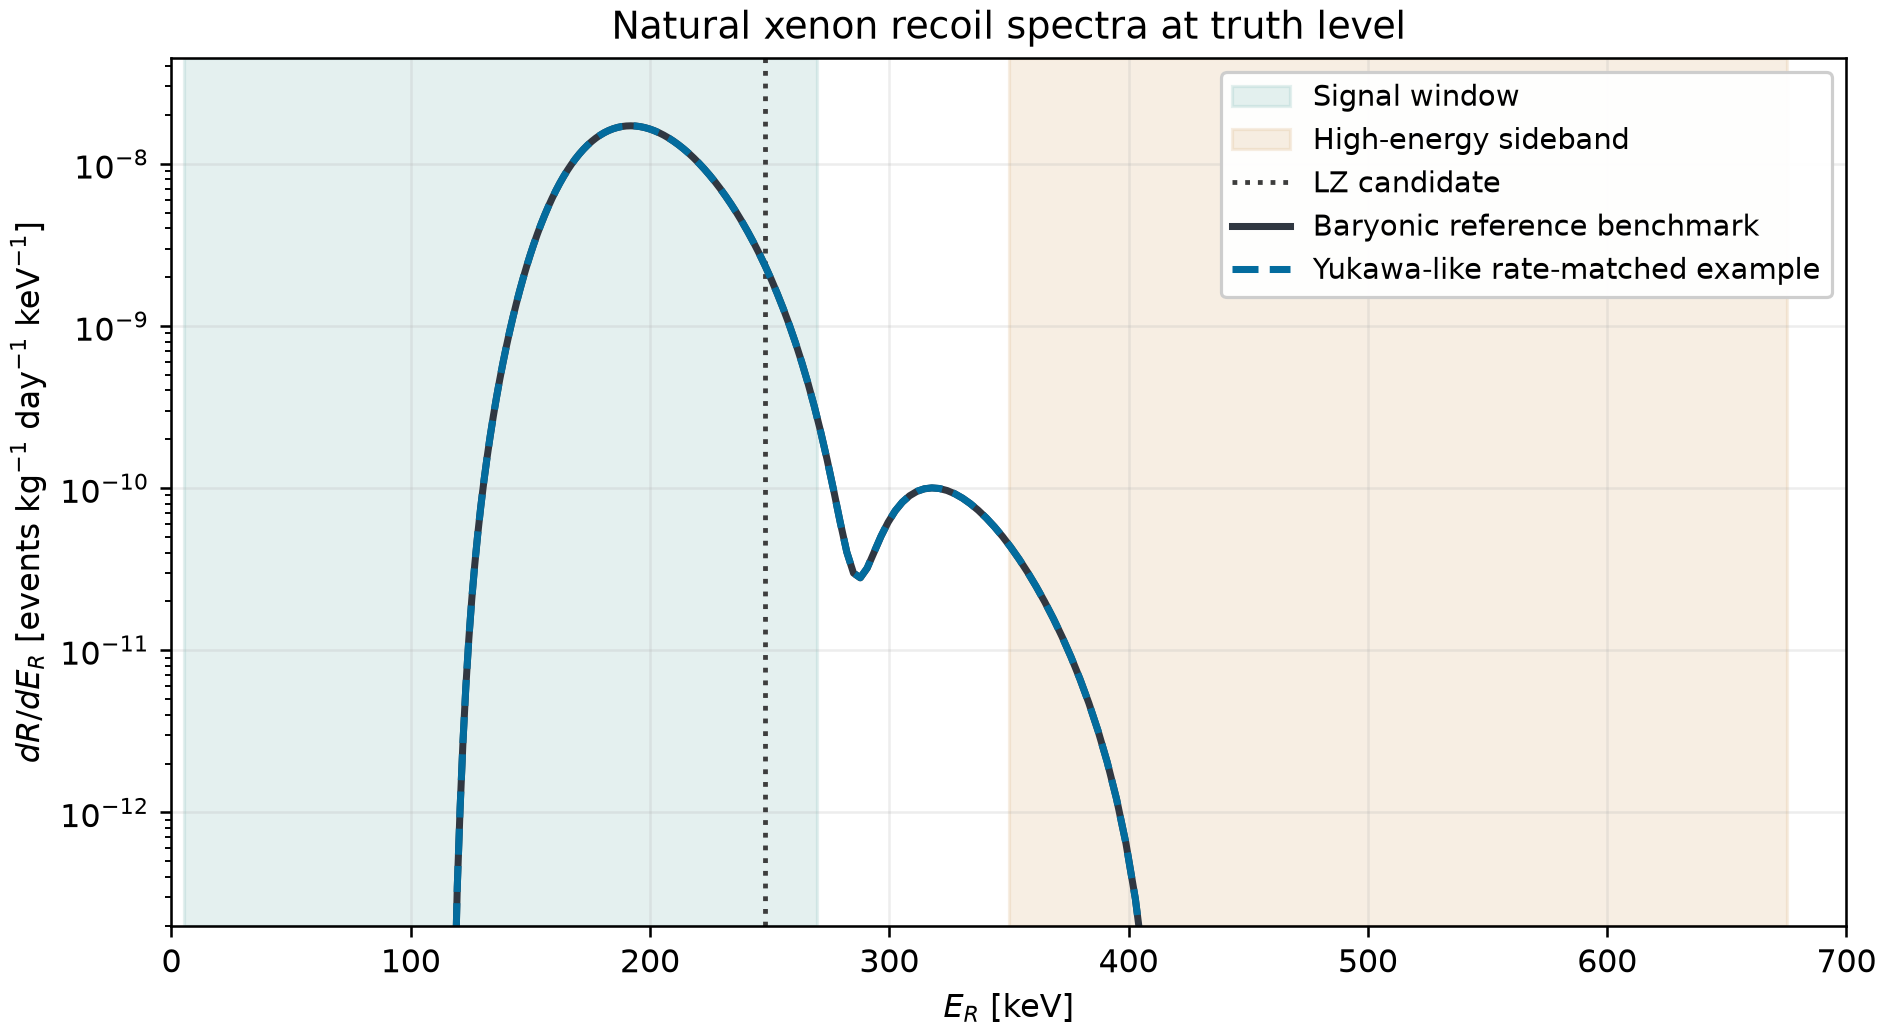
\includegraphics[width=\linewidth]{figures/01_xenon_recoil.png}
\caption{Truth-level differential recoil rates in events kg$^{-1}$ day$^{-1}$ keV$^{-1}$. Both models use $m_\chi=35$ GeV and $M_V=30$ GeV. For the mass-weighted model, $g_t=0.12763$ and $g_\chi=0.29779$ reproduce the reference yield. The vertical line marks the reconstructed recoil energy of the LZ candidate, and shading marks the integration windows.}
\label{fig:recoil}
\end{figure}

Eq.~\eqref{eq:recoil} determines the normalization of the recoil spectrum. In the contact limit $q\ll M_V$, the squared propagator gives $1/M_V^4$, and the tree-level nuclear coupling $Q_A$ is proportional to $g_t$. At fixed $m_\chi$, mass splitting, and halo model, the integrated yield therefore scales as $f_2\kappa^2$, where $\kappa=g_tg_\chi/M_V^2$ and $f_2$ is the present-day local fraction of dark matter in the heavier state.

For each $m_\chi$, let $\kappa_0(m_\chi)$ be the coupling combination that gives $N_0=1.12044$ truth-level events at tree level with $f_2=0.5$. The target yield in units of $N_0$ is $r=N_{\rm ROI}^{\rm truth}/N_0$. We define $K_\gamma(m_\chi,d_\gamma)$ as the ratio of the integrated yield with photon mixing to the tree-level yield in the same window, with $m_\chi$, $\kappa$, and $f_2$ held fixed.

\begin{equation*}
\frac{N_{\rm ROI}^{\rm truth}}{N_0}=\frac{f_2}{0.5}\left[\frac{\kappa}{\kappa_0(m_\chi)}\right]^2K_\gamma(m_\chi,d_\gamma).
\end{equation*}

Setting the yield ratio to the chosen $r$ and solving for $\kappa$ gives

\begin{equation}
\label{eq:yield}
\kappa=\kappa_0(m_\chi)\sqrt{\frac{r}{K_\gamma(m_\chi,d_\gamma)}\frac{0.5}{f_2}},\qquad
g_\chi=\frac{M_V^2}{g_t}\kappa.
\end{equation}

Integrating the spectrum separately at each mass gives $\kappa_0(35,40,44\,\mathrm{GeV})=(4.223,5.665,7.202)\times10^{-5}\ \mathrm{GeV}^{-2}$. As the dark matter mass increases, the characteristic recoil energy approaches the upper edge of the window, and a larger coupling product is needed to reproduce the reference yield. At fixed spectral shape, the normalization scales with $r/f_2$. We set $r=1$ for the reference yield and vary it over the prescribed range $r\in[0.75,1.25]$ to test the effect of the normalization. This range carries no LZ confidence level. We obtain the 95\% CL limits by fitting the CMS monojet likelihood in Section~\ref{sec:monojet_method}.

\section{Thermal abundance and physical branches}
\label{sec:abundance}

We assume a standard thermal history and chemical equilibrium between the two states during freeze-out. Their total number density $n=n_1+n_2$ obeys

\begin{equation}
\label{eq:boltzmann}
\begin{aligned}
\dot n+3Hn&=-\langle\sigma_{\rm eff}v\rangle[n^2-(n^{\rm eq})^2],\\
\langle\sigma_{\rm eff}v\rangle
&=\sum_{i,j=1,2}\frac{n_i^{\rm eq}n_j^{\rm eq}}{(n^{\rm eq})^2}\langle\sigma_{ij}v\rangle .
\end{aligned}
\end{equation}

The two dark states have the same spin degeneracy. In the nonrelativistic limit their equilibrium number densities satisfy

\begin{equation*}
\frac{n_2^{\rm eq}}{n_1^{\rm eq}}\simeq\left(\frac{m_2}{m_1}\right)^{3/2}e^{-\Delta m/T}.
\end{equation*}

The freeze-out temperature $T_f$ is much larger than the splitting $\Delta m$, so the Boltzmann factor $e^{-\Delta m/T_f}$ is close to unity. Each state therefore contributes about half of the equilibrium number density at freeze-out. The present-day local fraction $f_2$ also depends on late state conversion and the lifetime of the heavier state (Appendix~\ref{sec:matching}).

Each coannihilation through $\chi_1\chi_2\to V^*\to b\bar b,c\bar c$ consumes one particle of each state and reduces the total number by two. The $(1,2)$ and $(2,1)$ terms in Eq.~\eqref{eq:boltzmann} together contribute $2n_1^{\rm eq}n_2^{\rm eq}\langle\sigma_{12}v\rangle/(n^{\rm eq})^2$, or about $\langle\sigma_{12}v\rangle/2$ for equal equilibrium fractions. As the Universe cools and the actual density exceeds its equilibrium value, a larger coannihilation rate removes dark particles faster and lowers the relic abundance. Coannihilation is enhanced near the mediator resonance, making the abundance sensitive to $M_V$. At one on-shell benchmark with $m_\chi=35$ GeV, $b\bar b$ accounts for about $92\%$ of the coannihilation rate. Annihilation of two particles in the same dark state to $VV$ can set the abundance when that channel opens. \cite{griest1991,gondolo1991}

We compute the cross sections and solve for the total abundance with CalcHEP and micrOMEGAs 7.1.4, using \texttt{Fast=0} and \texttt{Beps=1e-9}. We assume that the two states together account for the full Planck dark matter abundance $\Omega_ch^2=0.1200\pm0.0012$. \cite{micromegas2024,planck2020}

At fixed $m_\chi$, Eq.~\eqref{eq:yield} gives the coupling and propagator factor for coannihilation as

\begin{equation}
\label{eq:propagator}
\frac{(g_tg_\chi)^2}{(M_V^2-s)^2+M_V^2\Gamma_V^2}
=\frac{\kappa^2 M_V^4}{(M_V^2-s)^2+M_V^2\Gamma_V^2}.
\end{equation}

Changing $g_\chi$ affects the thermal average through the mediator width. Changing $M_V$ also shifts the resonance relative to the energies accessible at freeze-out. At $m_\chi=35$ GeV, $g_\chi=0.18$, and $M_V\simeq87.56$ GeV, the local logarithmic slope of the abundance with respect to the mediator mass is about $0.158\ \mathrm{GeV}^{-1}$. In this slice, the Planck $\pm2\sigma$ interval corresponds to $M_V\simeq87.43$--$87.68$ GeV. When we vary $m_\chi$ as well, the yield and abundance conditions define multiple two-dimensional surfaces in the four-dimensional parameter space. More than one dark matter mass can satisfy both conditions at the same $(M_V,g_t)$.

\begin{figure*}[tbp]
\centering
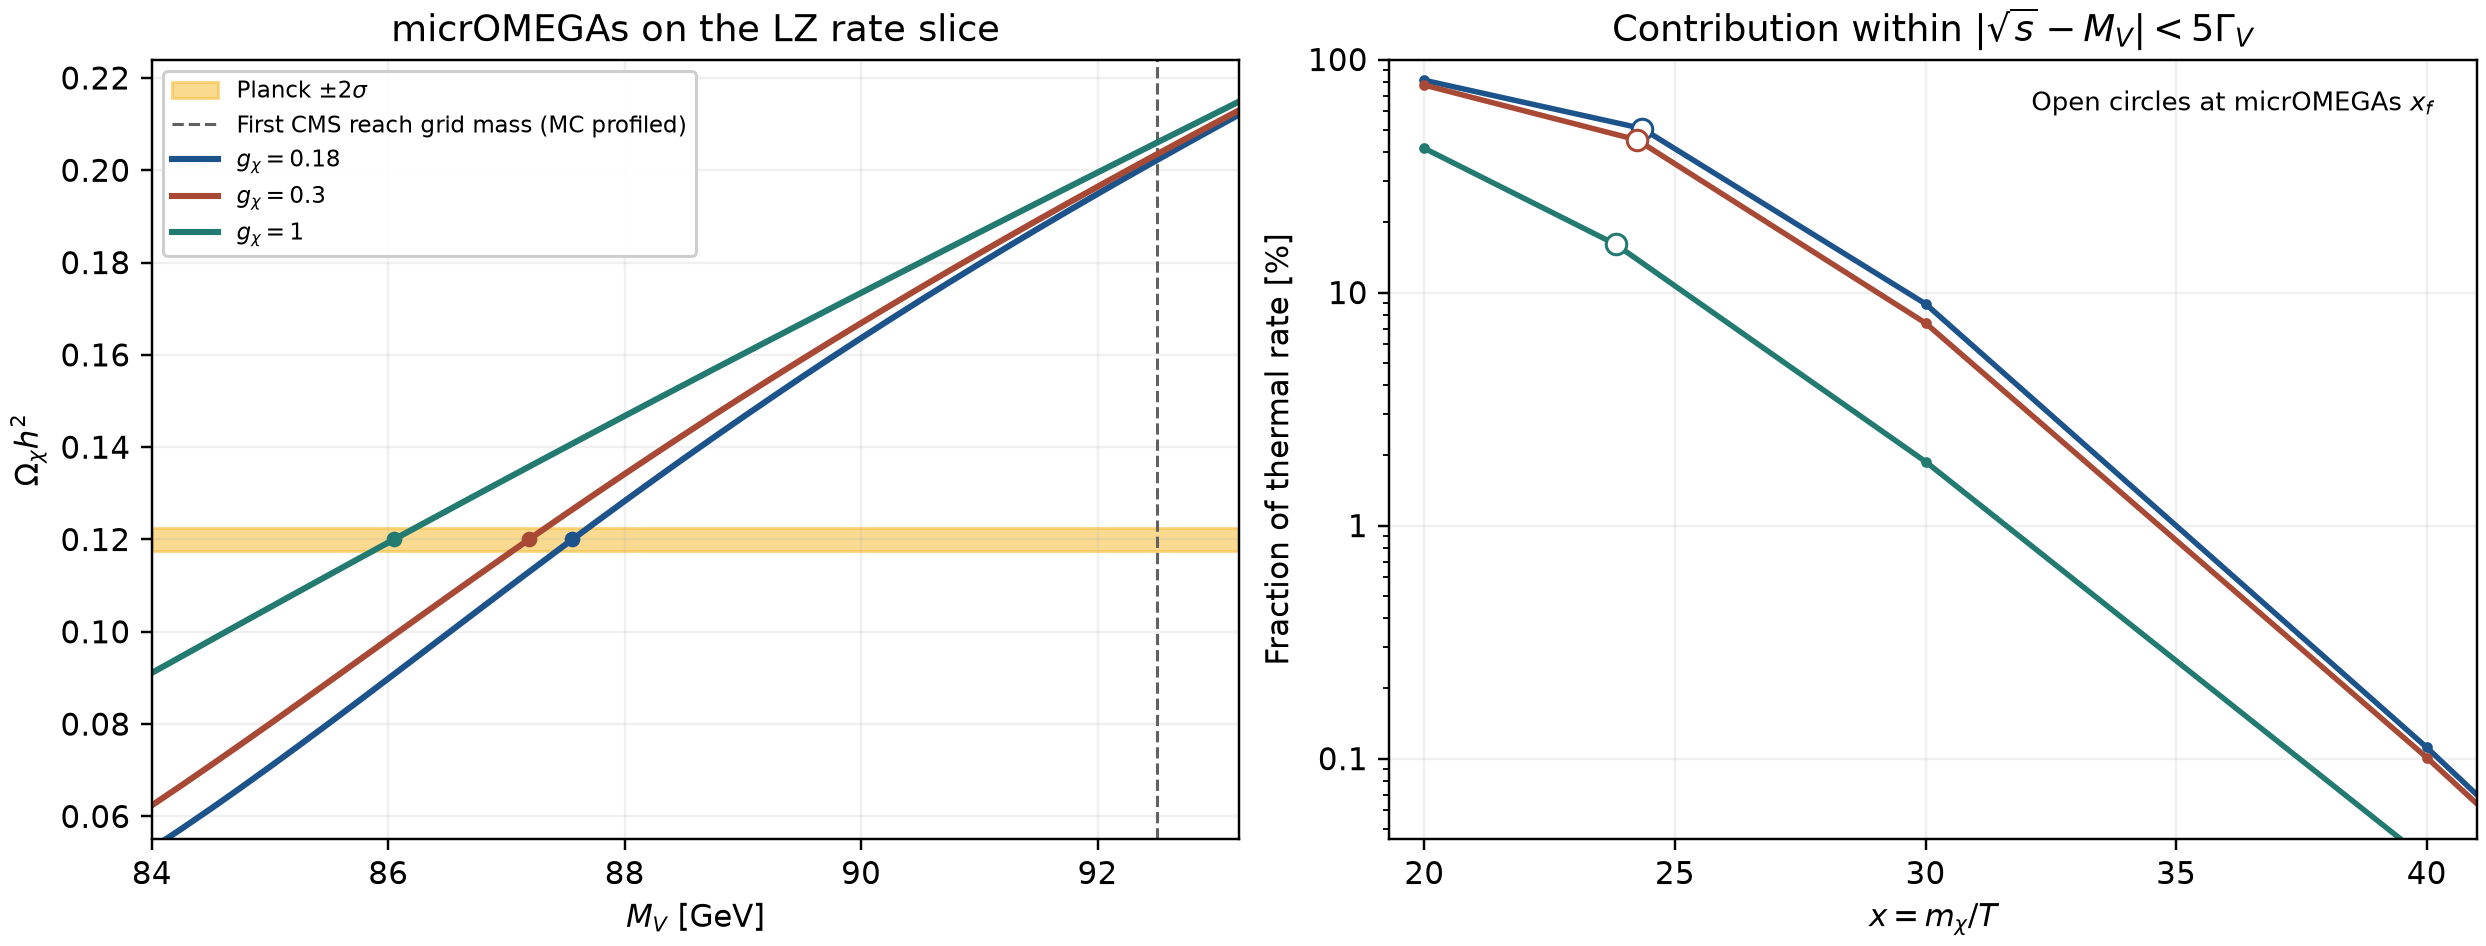
\includegraphics[width=\linewidth]{figures/02_relic_slope.png}
\caption{The left panel fixes $m_\chi=35$ GeV. The right panel shows the contribution of the pole neighborhood to the instantaneous thermal average. Open symbols mark the freeze-out temperatures at the individual points.}
\label{fig:relic}
\end{figure*}

The main grid uses $r=1$, $f_2=0.5$, and $d_\gamma(0)=0$ and includes the finite spacelike photon-mixing contribution from $c,b,t$ quarks. At each $(M_V,g_t)$, we eliminate $g_\chi$ with Eq.~\eqref{eq:yield} and look for crossings of $\Omega_\chi h^2=0.1200$ on both sides of $M_V-2m_\chi-\Delta m=0$. The grid contains 35 mediator masses and 29 top couplings. We bracket roots at dark mass intervals of at most $1.10$ GeV and sample more finely near threshold.

We approximate the Planck measurement $\Omega_ch^2=0.1200\pm0.0012$ with a Gaussian. The difference in $-2\ln\mathcal L_\Omega$ from its value at the center is the squared deviation in units of the measurement uncertainty.

\begin{equation*}
-2\ln\frac{\mathcal L_\Omega(\Omega_\chi h^2)}{\mathcal L_\Omega(0.1200)}
=\left(\frac{\Omega_\chi h^2-0.1200}{0.0012}\right)^2.
\end{equation*}

For example, $0.1188$ and $0.1176$ lie $1\sigma$ and $2\sigma$ below the center, giving 1 and 4, respectively. To propagate the measurement uncertainty to the collider limits, we use five abundance targets, $0.1176,0.1188,0.1200,0.1212,0.1224$, at each of 11 representative coordinates. For each target we hold $(M_V,g_t)$ and the LZ yield ratio $r$ fixed, scan $m_\chi$, and use Eq.~\eqref{eq:yield} to obtain $g_\chi$ at each trial mass. We record the parameters of each branch where the calculated abundance reaches the target. We record a missing solution when a branch has no root within the scan range at that target. Section~\ref{sec:monojet_method} defines the CMS limit for solutions that meet the on-shell template criteria. Section~\ref{sec:monojet_results} reports the effects of varying the abundance and the target recoil yield.

\section{LHC production, reconstruction, and statistical analysis}
\label{sec:monojet_method}

\subsection{Truth cross sections and reconstruction}

The monojet signal includes the tree-level channels $q\bar q\to gV$ and $qg\to qV$ and their charge conjugates, as well as the finite closed-quark-loop contribution $gg\to gV$. For a pure vector current, the three-point amplitude $gg\to V$ cancels. With an extra gluon, the four-point amplitude can be nonzero. We sum the tree and loop cross sections because these contributions have distinct initial states. We calculate $pp\to t\bar tV$ at tree level. We use MadGraph5\_aMC@NLO 3.6.6 with \texttt{nn23lo1} at 13 TeV and evaluate 11 values of $M_V$. In the narrow-width approximation, the cross section for final state $X$ is

\begin{equation}
\label{eq:nwa}
\sigma_X=\sigma_X^{\rm prod}(M_V;g_t=1)\,g_t^2\,\mathrm{BR}(V\to\chi_1\chi_2).
\end{equation}

The hard-cut truth-level cross sections and the comparison with top-pair production are given in Appendix~\ref{sec:top}. \cite{cox2016,alwall2014,hirschi2015}

We build reconstructed monojet templates with Pythia 8.312 and Delphes 3.5.0, treating the on-shell $V$ as invisible. Both samples start at generator-level $p_T^j=100$ GeV. To increase statistics in the tails, we generate additional tree and loop samples starting at 350 and 480 GeV, respectively, then combine the samples in mutually exclusive generator-level intervals. At $M_V=120$ GeV we add a loop-sample boundary at 230 GeV. Our reconstruction cuts approximate CMS EXO-20-004. We require the leading AK4 jet to satisfy $p_T>100$ GeV and $|\eta|<2.4$, and require $p_T^{\rm miss}>250$ GeV. We apply jet azimuthal cuts, lepton and photon vetoes, and heavy-flavor-related vetoes, and account for the 2018 HEM region. The data span three years and about $137\ \mathrm{fb}^{-1}$, with 22 monojet signal bins per year. \cite{pythia2022,delphes2014,cmsmonojet,albert2021}

\subsection{The 66-bin profile likelihood}

We use the public observations $n_i$, the background-only control-region prediction $\mathbf b$, its covariance $C_b$, and the signal $\mathbf s$ at each point to construct

\begin{equation}
\label{eq:likelihood}
\begin{aligned}
\mathcal L(\mu,\mathbf b',\mathbf s') &=
\prod_{i=1}^{66}\operatorname{Pois}(n_i\mid b_i'+\mu s_i')\\
&\quad\times G(\mathbf b';\mathbf b,C_b)\,G(\mathbf s';\mathbf s,C_s).
\end{aligned}
\end{equation}

We constrain the signal yields to be nonnegative and the Poisson means to be positive. The signal covariance $C_s$ includes the multinomial covariance of the simulated counts, cross-section integration errors, and a common $1.6\%$ luminosity uncertainty. We retain correlations across years when they share simulated events. Between mass nodes, we interpolate yields linearly and combine the covariances of independent samples with squared interpolation weights. For each branch, $\mu=1$ denotes its nominal prediction. We obtain $\mu_{95}$ by solving the asymptotic condition $CL_s=0.05$. The expected limits use an Asimov data set built from the central background prediction. The observed limits use the measured $n_i$ and a conditional background Asimov data set. The five expected quantiles describe background fluctuations. We propagate the relic-density uncertainty by solving again for each physical root. \cite{cmscovariance,cmsyields,cmssimplified,cowan2011,read2002}

We use the one-sided profile likelihood ratio

\begin{equation*}
\tilde q_\mu=-2\ln\frac{\mathcal L(\mu,\widehat{\widehat{\boldsymbol\theta}}_\mu)}{\mathcal L(\widehat\mu,\widehat{\boldsymbol\theta})}.
\end{equation*}

We set it to zero when $\widehat\mu>\mu$ and constrain $\widehat\mu\ge0$. With $a=\sqrt{\tilde q_{\mu,A}}$, the observed asymptotic statistic is

\begin{equation}
\label{eq:cls}
\begin{aligned}
CL_s(\mu)&=\frac{\Phi(-z_\mu)}{\Phi(a-z_\mu)},\\
z_\mu&=\begin{cases}\sqrt{\tilde q_\mu},&\tilde q_\mu\le a^2,\\
(\tilde q_\mu+a^2)/(2a),&\tilde q_\mu>a^2.\end{cases}
\end{aligned}
\end{equation}

For the expected bands, we solve $a=z-\Phi^{-1}[0.05\Phi(z)]$ on the nominal background Asimov data set for $z=-2,-1,0,1,2$. \cite{cowan2011}

Appendix~\ref{sec:validation} compares the 66-bin fit using official CMS vector templates with the published fit. It also compares the cutflow, acceptance, and MET spectra from independent simulation. CMS reports expected and observed vector mass boundaries of 2.198 and 1.957 TeV. The 66-bin reconstruction gives 2.208 and 1.941 TeV. The discrepancies are larger for individual observed limits at low masses. At the 2017 CMS vector benchmark with a 100 GeV mediator, independent fast simulation gives 62.9\% of the official absolute signal yield. This comparison limits the precision with which we can validate the acceptance used to locate the exclusion contour.

\section{Monojet results and stability}
\label{sec:monojet_results}

\subsection{Branch-resolved results at the central relic abundance}

At the reference yield $r=1$ with $f_2=0.5$ and $d_\gamma(0)=0$, Eq.~\eqref{eq:yield} fixes $g_\chi=g_\chi(m_\chi;M_V,g_t)$. Let $\mathcal D_\chi$ be the set of masses $20\le m_\chi\le100$ GeV for which Eq.~\eqref{eq:yield} gives $0.10\le g_\chi\le1.50$. At each $(M_V,g_t)$ we define

\begin{equation*}
\begin{gathered}
\mathcal S_{\rm on}(M_V,g_t) = \{m_\chi\in\mathcal D_\chi:\ \Omega_\chi h^2=0.1200,\\
M_V-m_1-m_2\ge5\Gamma_V,\quad \Gamma_V/M_V<0.03\}.
\end{gathered}
\end{equation*}

Where $\mathcal S_{\rm on}$ contains exactly one solution, the color shows the 95\% CL limit $\mu_{95}$ from CMS data alone for that branch. The black contour marks $\mu_{95}=1$. Gray marks coordinates without a unique on-shell solution satisfying the narrow-width criteria in the scan. An off-shell monojet limit would require templates from the full $pp\to j\chi_1\chi_2$ matrix element.

\begin{figure*}[tbp]
\centering
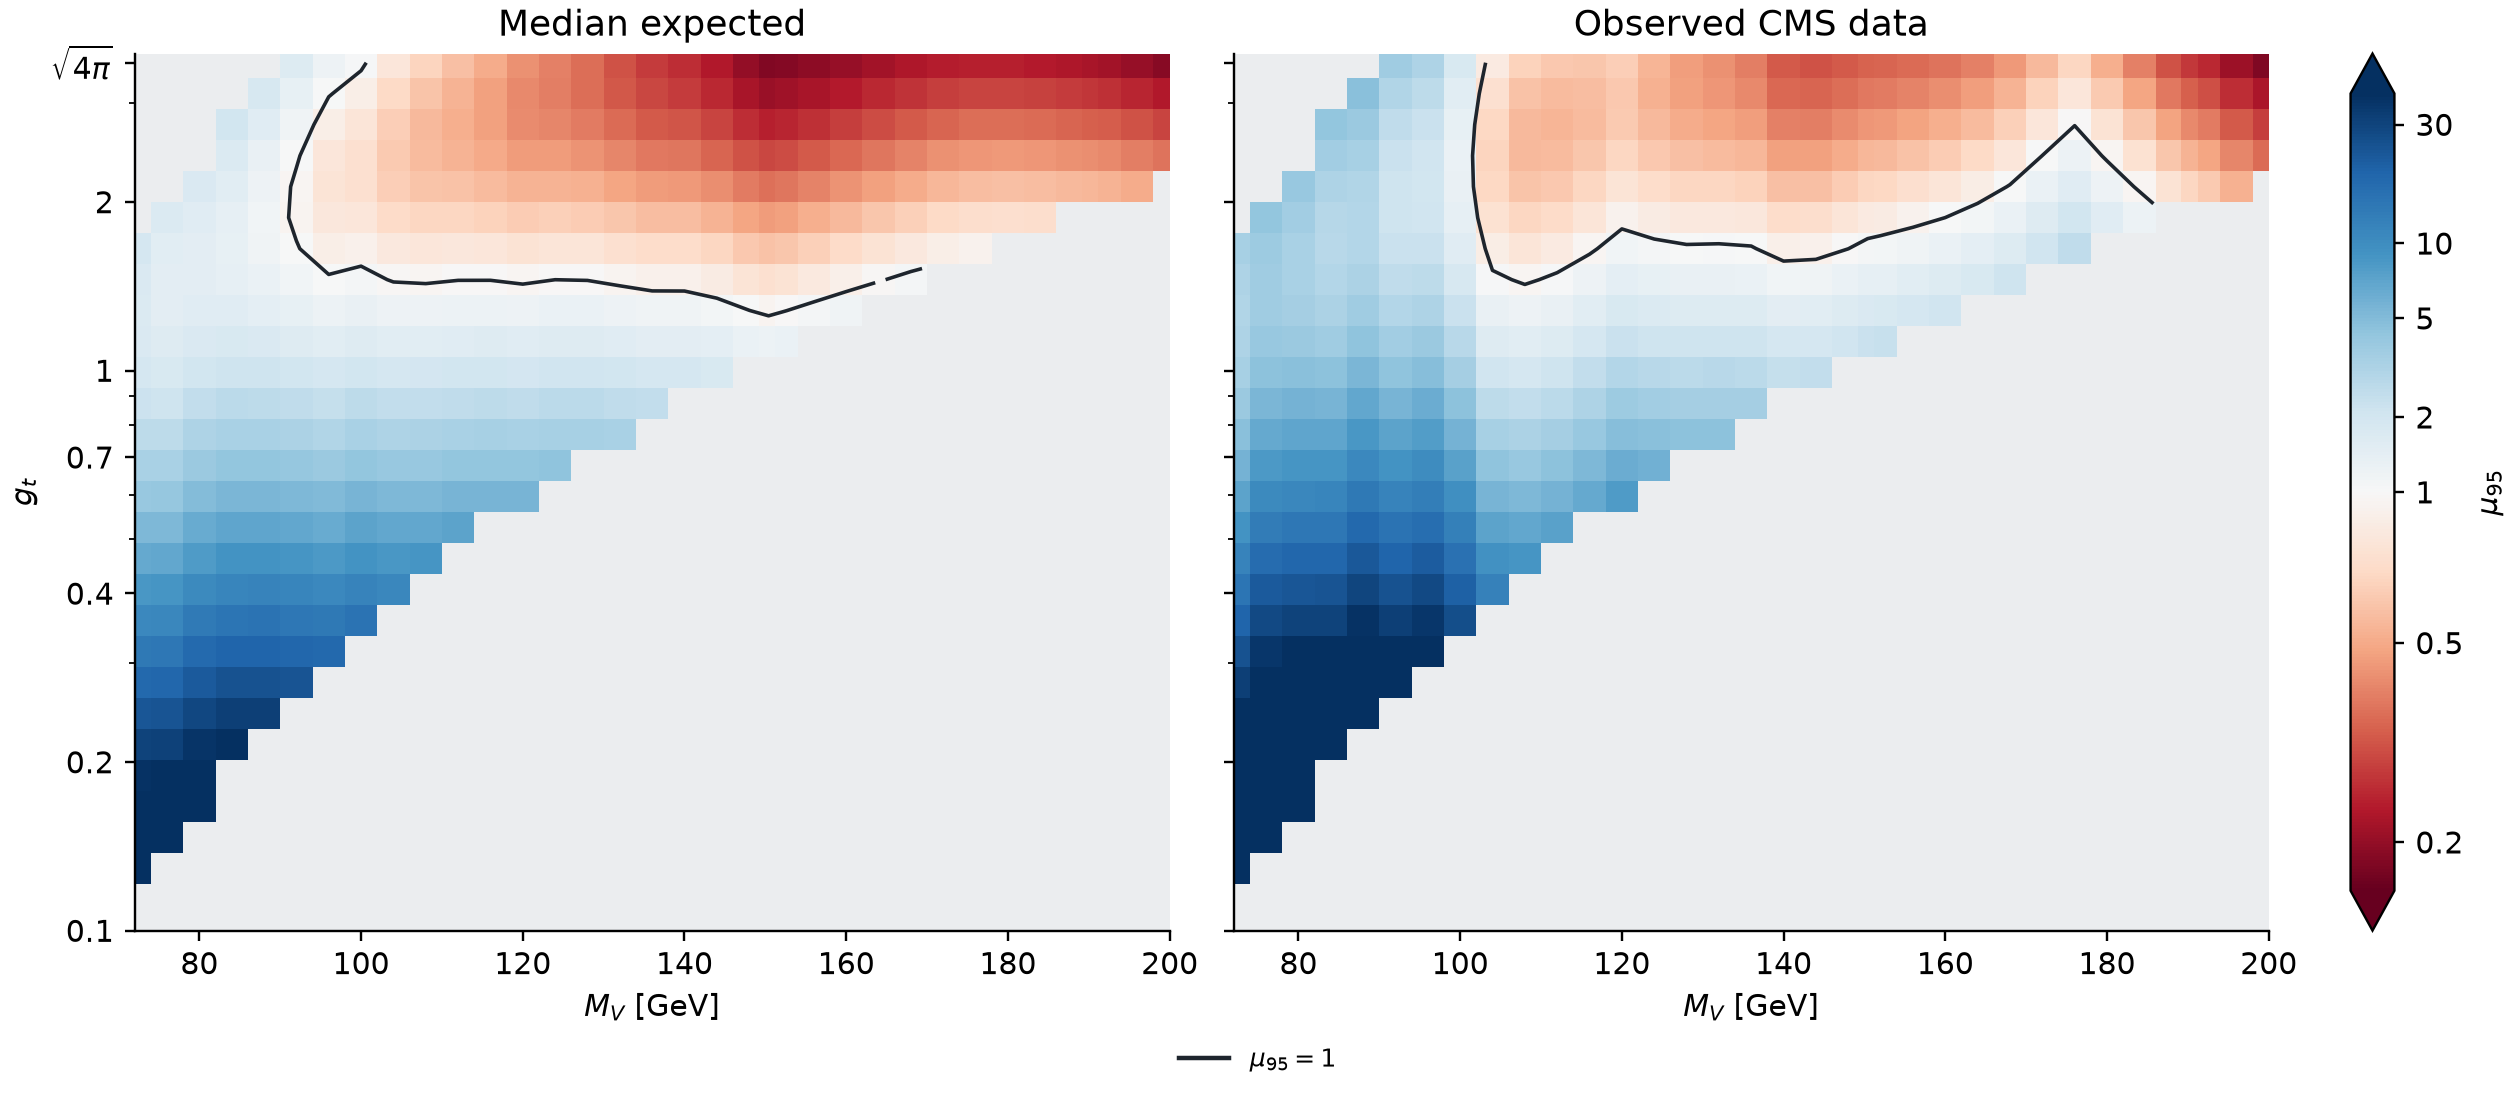
\includegraphics[width=\linewidth]{figures/04_cms_central_plane.png}
\caption{Expected and observed CMS monojet 95\% confidence-level limits on the unique branch satisfying the recoil-yield, central-abundance, and narrow-width conditions. The black contour marks $\mu_{95}=1$. Gray denotes coordinates with no unique in-scope solution.}
\label{fig:exclusion}
\end{figure*}

Of the 1,015 grid coordinates, 434 have a unique on-shell solution at the central relic abundance that satisfies the template requirements. With the reference templates in Fig.~\ref{fig:exclusion}, the expected and observed limits fall below unity at 208 and 151 points, respectively. The lowest sampled masses with $\mu_{95}<1$ are 92 and 104 GeV. These counts and masses depend on the grid spacing. At the interior point $(M_V,g_t)=(112\,\mathrm{GeV},2.747)$, the solution $(m_\chi,g_\chi)=(40.055\,\mathrm{GeV},0.260)$ gives expected and observed limits of $0.513$ and $0.540$. The smallest observed limit with the reference templates is $0.181$ at $(200\,\mathrm{GeV},\sqrt{4\pi})$. With pooled templates at three mass nodes, the number of observed limits below unity rises to 162, with 11 grid points crossing the exclusion contour (Appendix~\ref{sec:validation}). Section~\ref{sec:discussion} discusses the off-shell roots at lower masses.

At some mediator masses, monojet sensitivity is confined to a finite interval in $g_t$. At fixed masses and LZ yield, $g_\chi\propto g_t^{-1}$, so $\Gamma_{\chi_1\chi_2}=A/g_t^2$ and $\Gamma_{\rm SM}=Bg_t^2$, with $A,B$ constant on the slice. The signal factor in Eq.~\eqref{eq:nwa} is $g_t^2/(1+(B/A)g_t^4)$ and peaks where the two widths are equal. At larger $g_t$, the invisible branching fraction can decrease enough to offset the increase in production.

\begin{table*}[tbp]
\caption{Representative on-shell branches. The reference limits use $r=1$, $f_2=0.5$, $d_\gamma(0)=0$, and the central Planck abundance. The last column gives the observed limits after solving for the abundance again at each target yield. The upper scan boundary is $g_t=3.545$.}
\label{tab:benchmarks}
\begin{ruledtabular}
\begin{tabular}{rrrrrrr}
$M_V$ [GeV] & $g_t$ & $m_\chi$ [GeV] & $g_\chi$ & Expected $\mu_{95}$ & Observed $\mu_{95}$ & Observed, $r=0.75$--$1.25$ \\
\hline
80 & 0.503 & 33.027 & 0.482 & 6.891 & 15.58 & 15.55--15.64 \\
100 & 1.264 & 38.065 & 0.400 & 1.333 & 2.305 & 2.276--2.352 \\
120 & 3.073 & 41.116 & 0.284 & 0.412 & 0.607 & 0.570--0.664 \\
150.4 & 1.260 & 43.896 & 1.286 & 0.986 & 1.822 & 1.820--1.824 \\
150.4 & 3.545 & 43.896 & 0.457 & 0.184 & 0.340 & 0.329--0.357 \\
190.4 & 3.545 & 45.854 & 0.823 & 0.219 & 0.273 & 0.270--0.277 \\
\end{tabular}
\end{ruledtabular}
\end{table*}

\begin{figure}[tbp]
\centering
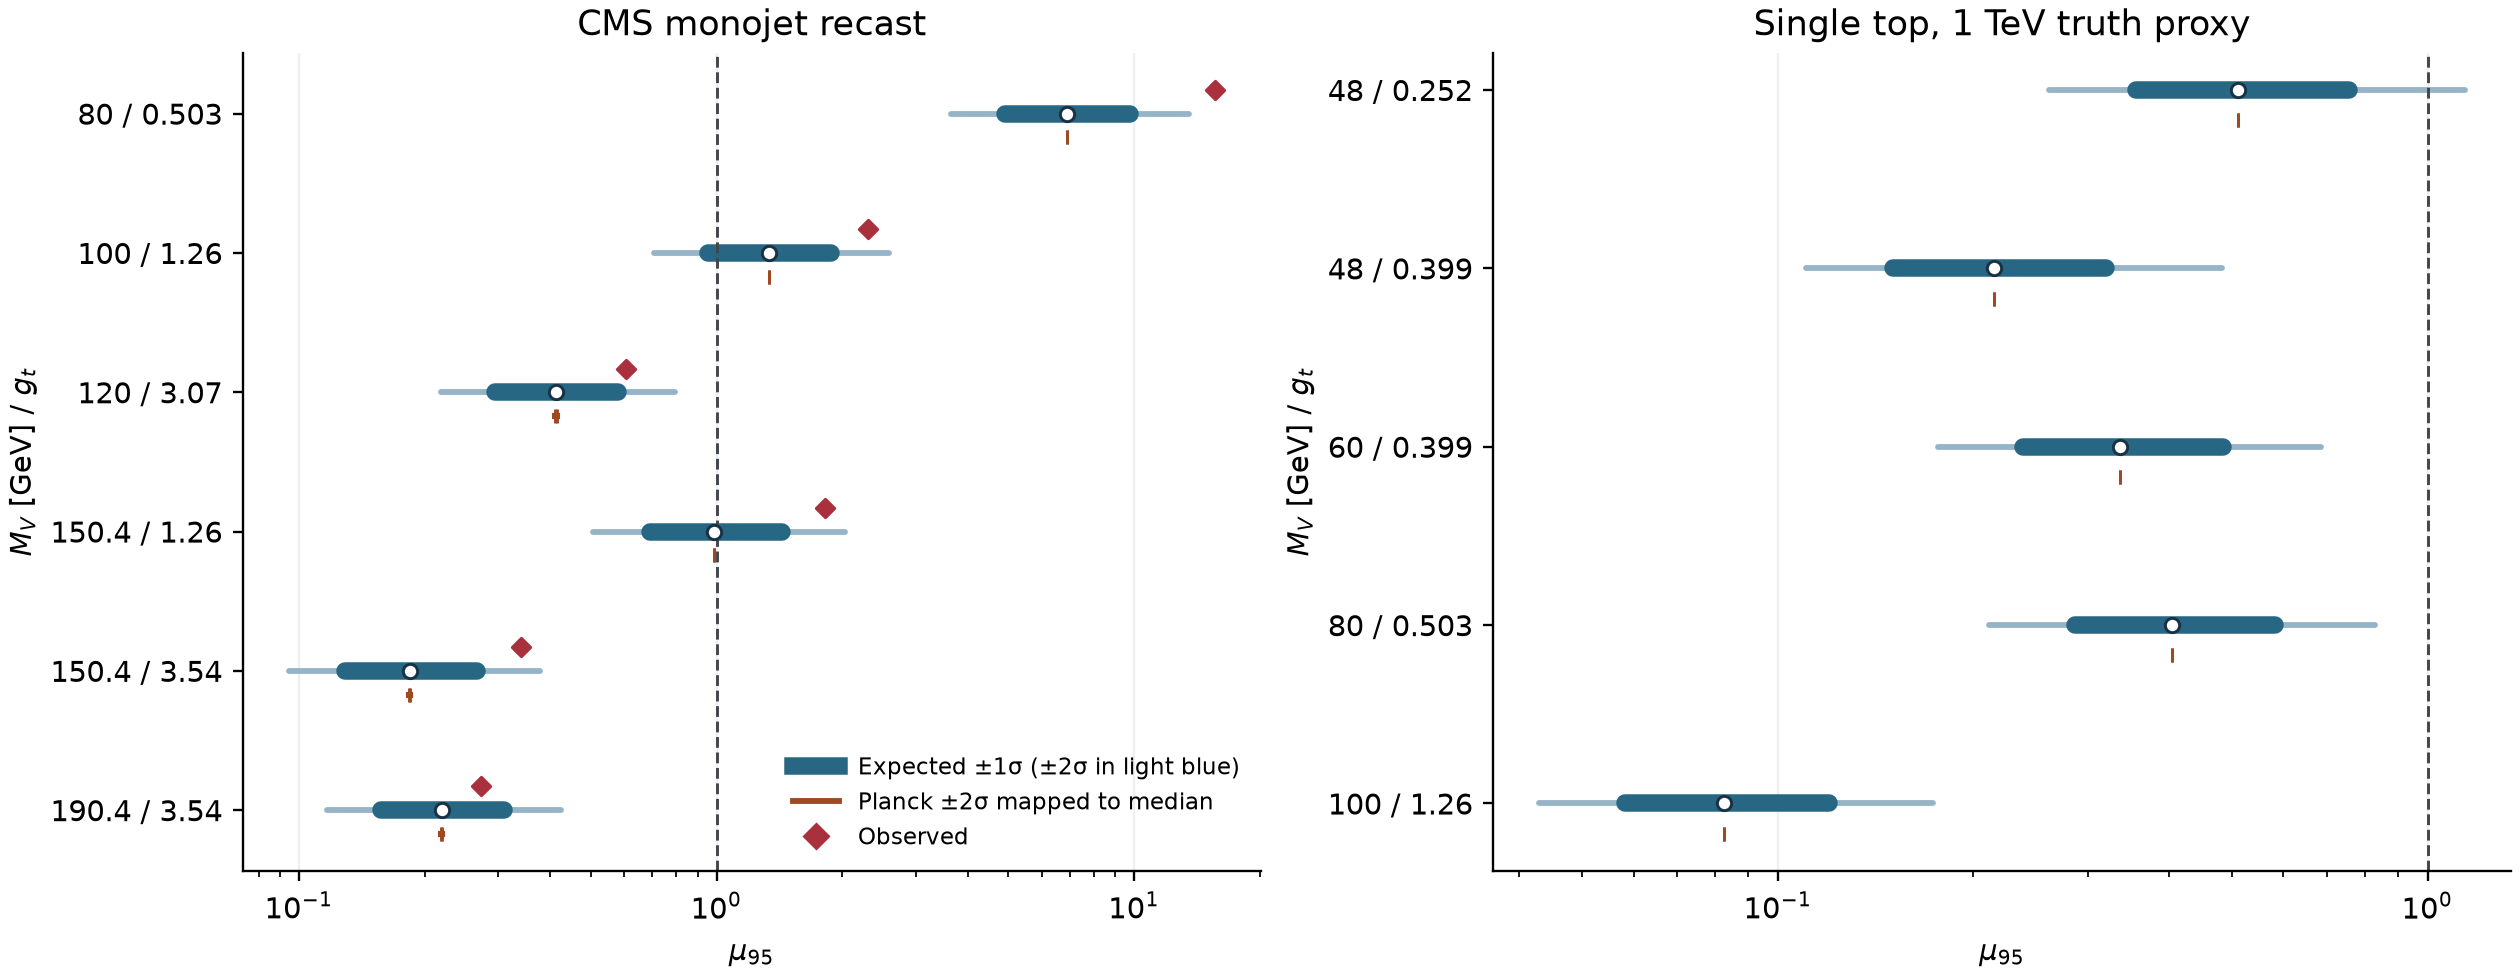
\includegraphics[width=\linewidth,trim=0 0 432bp 0,clip]{figures/05_collider_uncertainties.png}
\caption{Blue intervals show the $\pm1\sigma$ and $\pm2\sigma$ expected quantiles from background fluctuations. Brown marks show the effect of the Planck $\pm2\sigma$ measurement uncertainty on the median expected limit. Red diamonds mark observed limits.}
\label{fig:uncertainties}
\end{figure}

Using the procedure in Section~\ref{sec:abundance}, we find that varying the Planck abundance by $\pm2\sigma$ changes the median expected monojet $\mu_{95}$ by at most $0.44\%$ relative to the central-abundance result at the reference on-shell benchmarks. For example, at $M_V=150.4$ GeV, $g_t=1.260$, and $r=1$, the targets $0.1188,0.1200,0.1212$ give $(m_\chi/{\rm GeV},g_\chi)=(43.945,1.290),(43.896,1.286),(43.848,1.282)$, respectively. Across all five abundance targets, the median expected $\mu_{95}$ for this branch ranges from $0.98589$ to $0.98606$.

At the 120 GeV point in Fig.~\ref{fig:uncertainties}, propagating the abundance uncertainty gives median expected limits from $0.41056$ to $0.41415$. Background fluctuations give a $1\sigma$ expected band of $[0.295,0.581]$. Accounting for finite signal statistics and luminosity weakens the median expected limits by about $1.4\%$--$6.6\%$ compared with fits that fix the signal template. A model-specific covariance for scale and PDF uncertainties, production matching, and detector efficiencies remains to be determined.

\subsection{Low-energy photon mixing, the rate target, and the excited fraction}

\label{sec:low_energy}

Kinetic mixing with the photon gives the mediator $V$ an additional coupling to the electromagnetic current. We define $d_\gamma=e\epsilon_\gamma/g_t$, so the effective proton coupling receives a shift of $g_t d_\gamma$. The zero-momentum value $d_\gamma(0)$ is an independent matching input, which we set to zero in the main scan. Charged-quark loops give a finite correction relative to zero momentum. We retain the $c,b,t$ contribution $\delta d_{cbt}(-q^2)$ from Appendix~\ref{sec:matching}. \cite{deramo2016,forner2026}

With a common Helm form factor, only the protons contribute to the electric charge term, so photon mixing shifts $Q_A/g_t$ by $Z[d_\gamma(0)+\delta d_{cbt}(-q^2)]$. For $^{131}$Xe, the tree-level charge is $Q_A/g_t\simeq8.05\times10^{-3}$ and $Z=54$. The mixing contribution can therefore nearly cancel the tree-level amplitude at $d_\gamma(0)\simeq-1.49\times10^{-4}$. At the reference value $d_\gamma(0)=0$ and $m_\chi=35$ GeV, the retained momentum-dependent correction reduces the integrated rate in the recoil window by about $0.077\%$.

At $m_\chi=35$ GeV and fixed couplings, $d_\gamma(0)=-7\times10^{-6}$ and $+7\times10^{-6}$ give rates of $0.908$ and $1.095$ times the tree-level rate, respectively. Matching the same reference yield then requires $\kappa/\kappa_0=1.050$ and $0.956$, respectively. Near cancellation, this ratio rises to about $56.5$. In that case we find no solution at the central Planck abundance within the scanned coupling ranges at the 11 coordinates tested.

Figure~\ref{fig:mixing} compares the required coupling and the recoil spectra.

Varying the target yield over $r=0.75$--$1.25$ changes the median expected monojet limit by at most $9.4\%$ at the points tested. Reducing $f_2$ alone to 0.45 or 0.30 changes it by up to $3.0\%$ and $12.8\%$, respectively. Varying only the low-energy mixing within $|d_\gamma(0)|\le7\times10^{-6}$ changes it by at most $2.8\%$. At the 120 GeV benchmark, the choices $(d_\gamma(0),r,f_2)=(+7\times10^{-6},0.75,0.50)$ and $(-7\times10^{-6},1.25,0.45)$ give median expected limits of $0.465$ and $0.367$, respectively. Appendix~\ref{sec:matching} discusses how late downscattering and the excited-state lifetime affect the present-day fraction.

In a separate check at $r=2$, we solve again for the central Planck abundance. The three sensitive benchmarks in Table~\ref{tab:benchmarks} at $M_V=120,150.4,190.4$ GeV still give observed $\mu_{95}<1$, with limits of $0.507,0.310,0.265$, respectively.

At the other representative point with $M_V=150.4$ GeV and $g_t=1.260$, increasing $r$ from 1 to 2 moves the central-abundance solution to $g_\chi=1.498$, close to the scan boundary $g_\chi=1.50$. The invisible branching fraction rises from $0.9922$ to $0.9944$, and the observed $\mu_{95}$ changes from $1.822$ to $1.818$, remaining above the exclusion threshold. At $r=2$ we find no solution on this branch within the scan range for the lower abundance targets $0.1188$ and $0.1176$, so no CMS limits are available at those two targets.

Figure~\ref{fig:rate} shows how the limits vary with the target yield.

\section{Discussion of top-associated production}
\label{sec:discussion}

At a fixed $(M_V,g_t)$, the on-shell and off-shell relic solutions can give different signals in $t\bar t+\mathrm{MET}$. We compute the full four-body final state below the invisible-decay threshold and give representative truth-level rates in Appendix~\ref{sec:top}. A CMS exclusion in the all-hadronic two-$b$-tag category requires signal acceptance after top decays and a likelihood with background constraints independent of the signal-region counts. The single-top estimate in Appendix~\ref{sec:top} is sensitive to the partonic-energy cut. \cite{cmstop}

\section{Conclusions}
\label{sec:conclusions}

In this broken-phase vector model, light-quark couplings set the leading coherent xenon recoil amplitude, and heavy-quark couplings drive production at the LHC. For small photon mixing, fixed dark-state splitting, and a standard thermal history, the CMS Run 2 monojet recast excludes some on-shell solutions that reproduce the reference recoil yield and central Planck abundance. Their observed 95\% CL limits satisfy $\mu_{95}<1$. The three sensitive benchmarks remain excluded when the truth-level yield target varies by $25\%$. For lighter mediators, on-shell and off-shell relic solutions can occur at the same mediator mass and top coupling. The strong dependence on the partonic-energy cut limits the single-top result to an exploratory estimate. A joint confidence region would require an event-level LZ likelihood for the model, theoretical uncertainties on the abundance, and profiling over shared parameters.



\section*{Data availability}
The experimental inputs are available through the LUX-ZEPLIN and CMS public
data releases \cite{lzdata,cmscovariance,cmsyields,cmssignal,cmscutflow}.
The model files, analysis sources, public-input snapshots, binned signal
templates, numerical scans, and reproduction instructions are available at
\url{https://github.com/Jim11451/lz_paper}, tagged
\texttt{reproducibility-2026.11.19}. The reproduction package records the
software dependencies and distinguishes offline likelihood validation from
fresh event-generation and detector-simulation jobs.

\clearpage
\onecolumngrid
\appendix
\numberwithin{equation}{section}

\section{Xenon recoil and matching checks}
\label{sec:matching}

\begin{figure}[tbp]
\centering
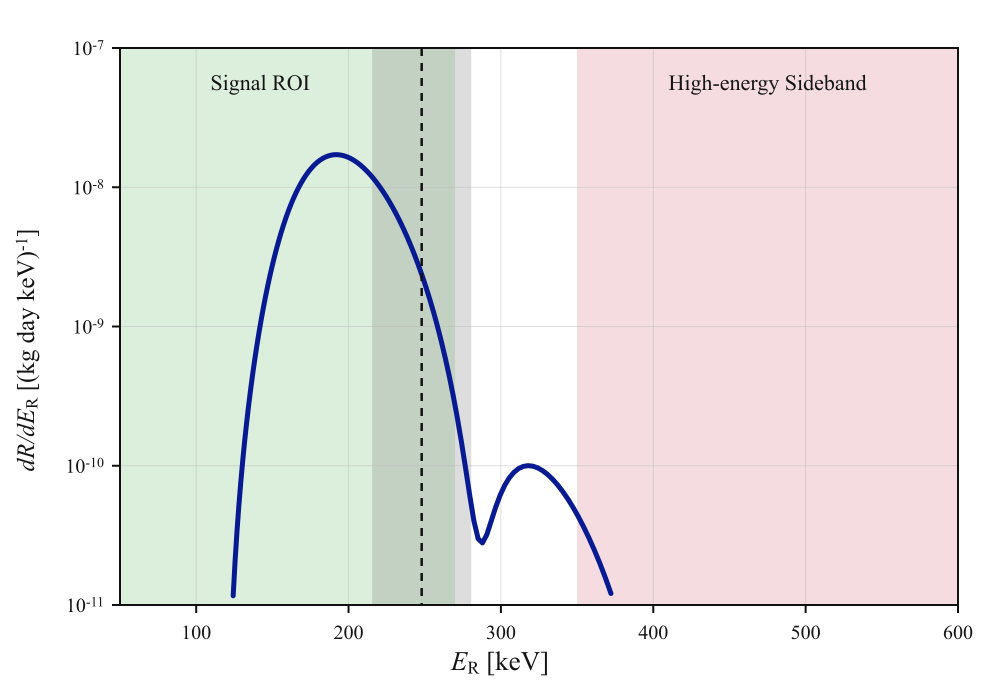
\includegraphics[width=.58\linewidth]{figures/a01_original_recoil.png}
\caption{Independent reproduction of the universal-vector reference benchmark, used to check the recoil shape and units.}
\label{fig:reference_recoil}
\end{figure}

After subtraction at zero momentum, the finite heavy-quark contribution to photon mixing is

\begin{equation}
\label{eq:finite_mixing}
\begin{aligned}
\delta d_{cbt}(s)&=-\frac{2\alpha}{\pi}\sum_{q=c,b,t}N_cQ_q\frac{\widehat m_q}{m_t}\\
&\quad\times\int_0^1 dx\,x(1-x)\log\left[1-\frac{s x(1-x)}{\widehat m_q^2}-i0\right].
\end{aligned}
\end{equation}

\begin{figure}[tbp]
\centering
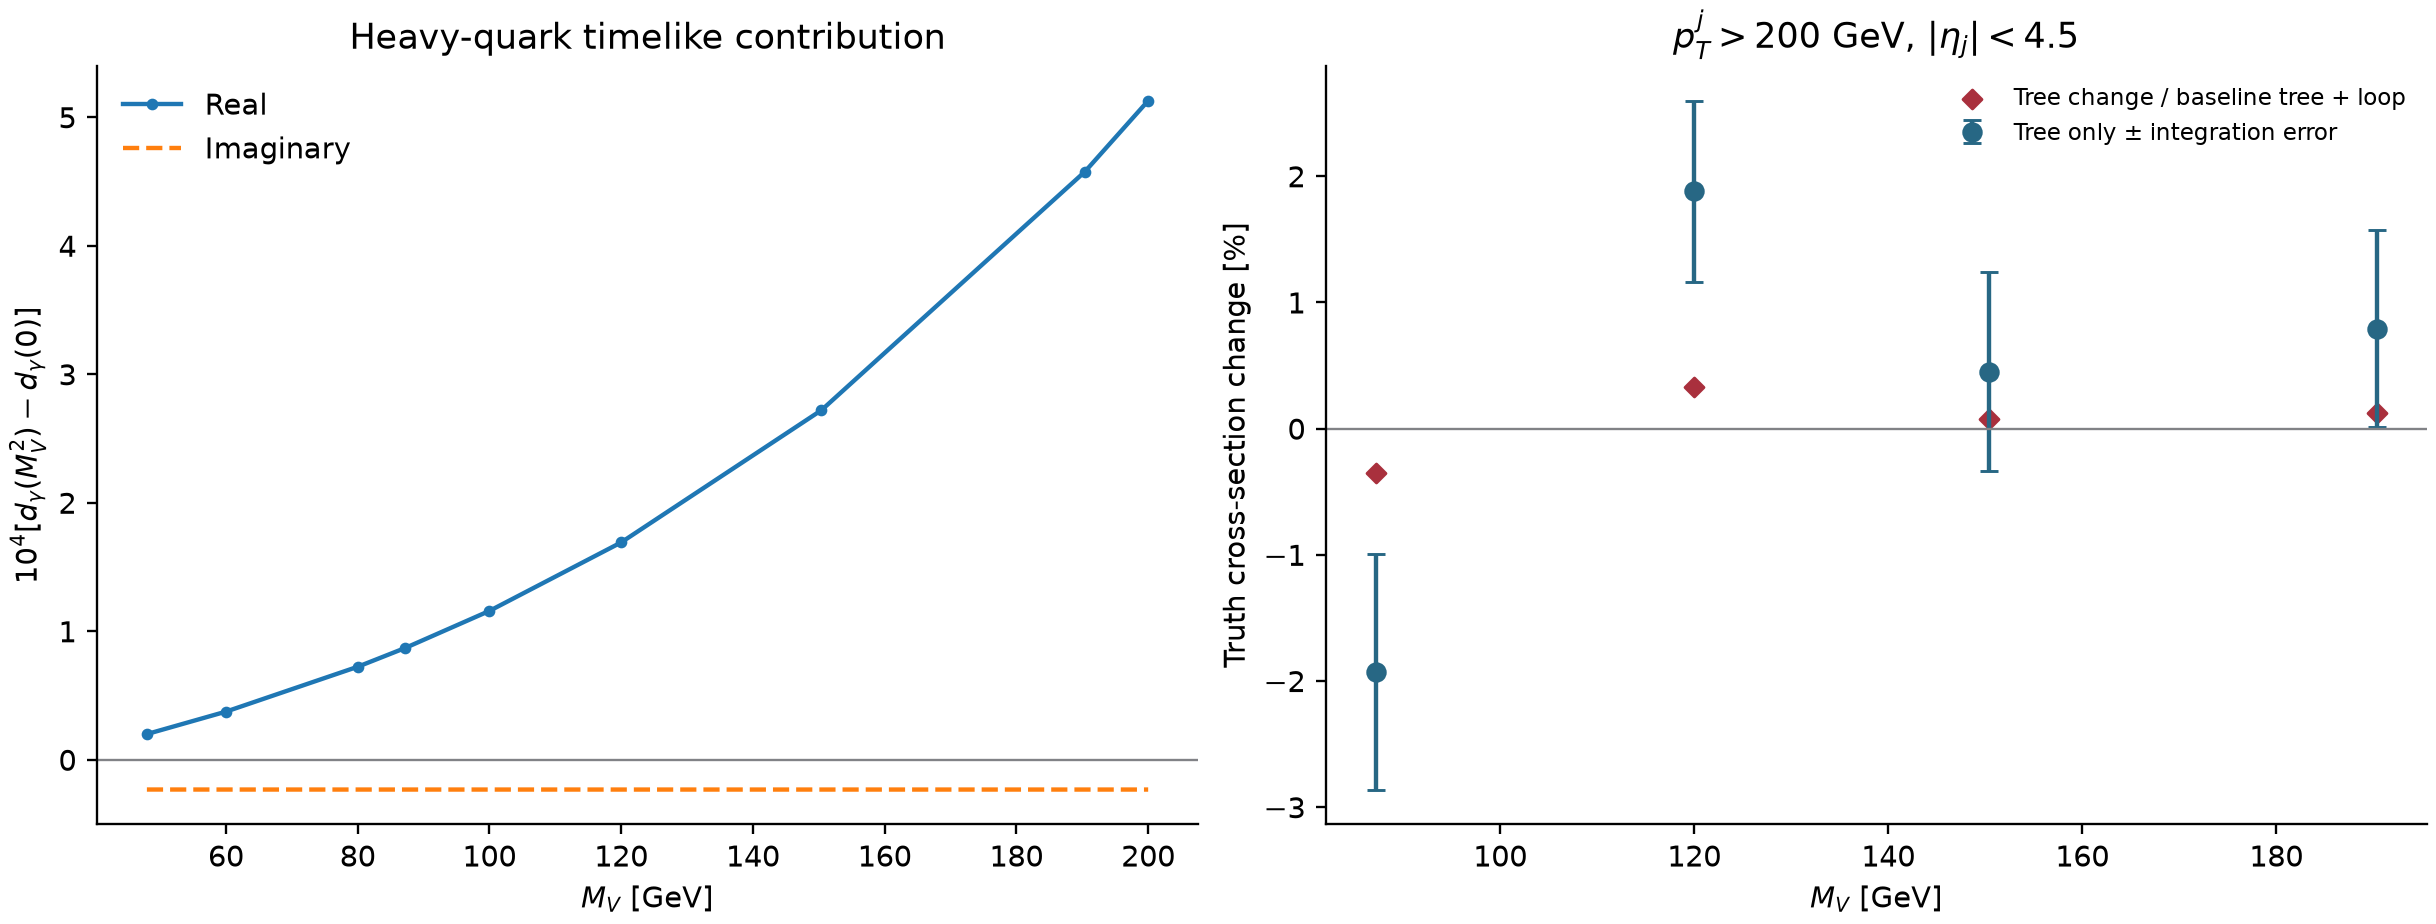
\includegraphics[width=.86\linewidth]{figures/a02_timelike_mixing.png}
\caption{At four on-shell masses we include $\delta d_{cbt}(M_V^2)$ in the $pp\to Vj$ tree amplitude. For $p_T^j>200$ GeV, the tree cross section changes by about $2\%$ or less. Relative to the original tree-plus-loop cross section, the shift is below $0.4\%$. For the relic calculation, we approximate the finite term by its real part evaluated at the dark-pair threshold or at the mediator pole. The largest shifts in $\Omega h^2$ across the four points are $1.12\times10^{-4}$ and $4.64\times10^{-4}$, respectively. Lowering \texttt{Beps} by two orders of magnitude changes the abundance by less than $2\times10^{-11}$ at three numerical benchmarks.}
\label{fig:timelike}
\end{figure}

\begin{figure}[tbp]
\centering
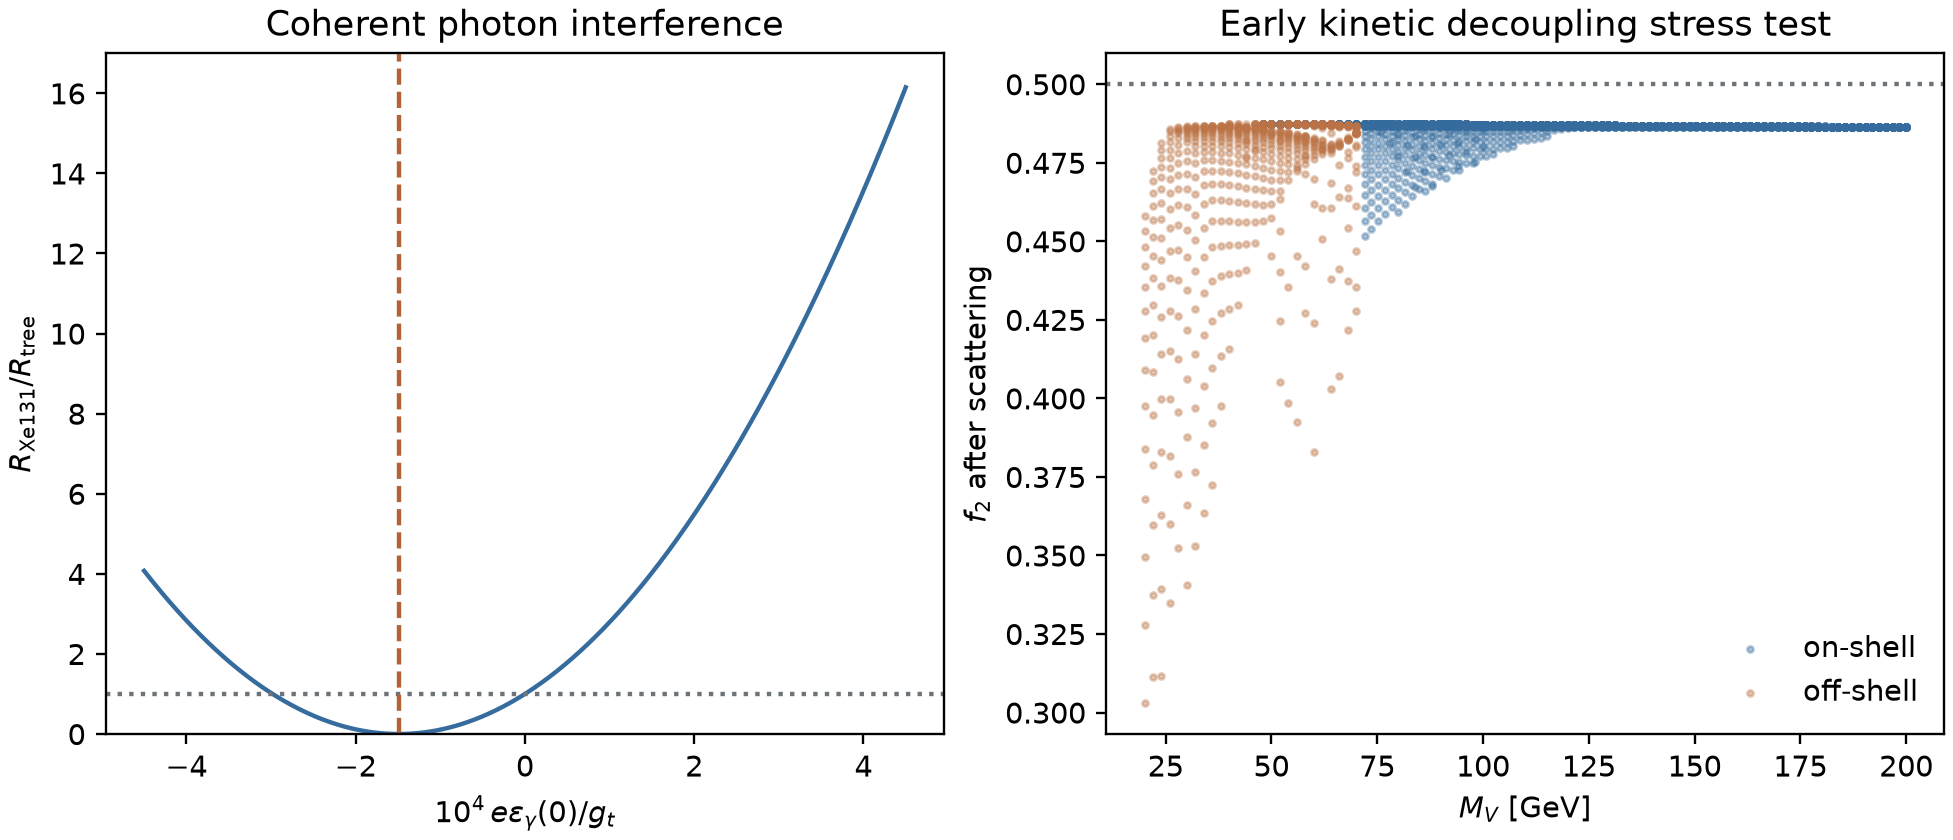
\includegraphics[width=.86\linewidth]{figures/a03_excited_fraction.png}
\caption{The conversion $\chi_2\chi_2\leftrightarrow\chi_1\chi_1$ can change the excited-state fraction after chemical freeze-out. In the standard thermal histories tested, with additional decay suppressed and the Standard Model bath included, the minimum at the on-shell benchmarks is $f_2\simeq0.45$ and falls to about $0.30$ at some off-shell benchmarks. The splitting $\Delta m<2m_e$ closes the electron-pair decay channel. Independent $V$--$Z$ mixing or a transition dipole can still affect the lifetime. \cite{gemmell2026,carrillo2022}}
\label{fig:fraction}
\end{figure}

After the total abundance freezes out, detailed balance for dark-state conversion gives $\dot f_2=-n_\chi\langle\sigma v\rangle_{22\to11}[f_2^2-e^{-2\Delta m/T_\chi}(1-f_2)^2]$, where $T_\chi$ is the dark-sector kinetic temperature. We model conversion with Born contact scattering and vary the assumptions about kinetic decoupling. The resulting $f_2$ values serve as benchmarks for those thermal histories.

\begin{figure}[tbp]
\centering
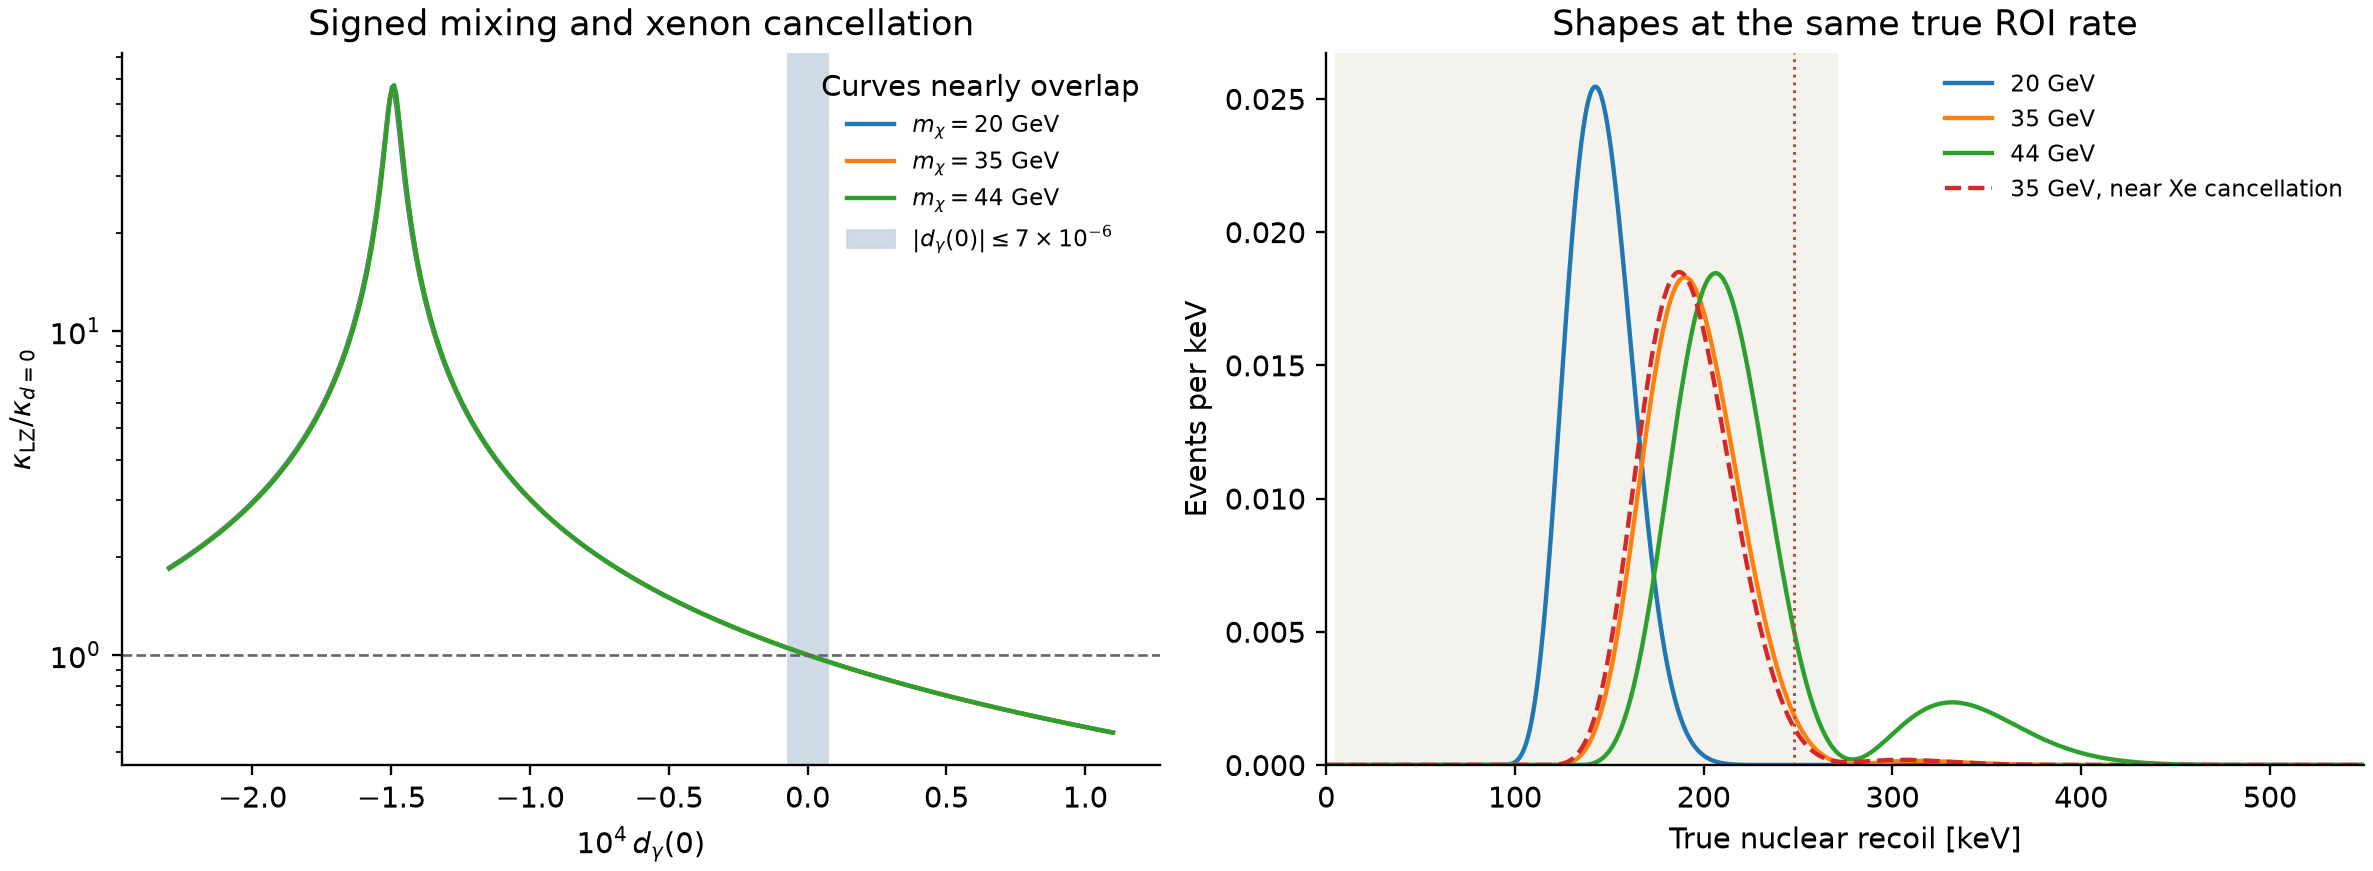
\includegraphics[width=.86\linewidth]{figures/06_matching_and_spectra.png}
\caption{The left panel shows how photon mixing changes the coupling required to match the yield. The right panel compares spectra with the same integrated truth-level yield. After Gaussian smoothing with a width of 32.5 keV, the signal densities near 248 keV at $m_\chi=20,35,44$ GeV are approximately $2.75\times10^{-4}$, $4.54\times10^{-3}$, and $6.98\times10^{-3}$ events/keV. The energy-spectrum approximation uses Gaussian smoothing alone. The LZ S1/S2 response and backgrounds enter an event-level analysis.}
\label{fig:mixing}
\end{figure}

\begin{figure}[tbp]
\centering
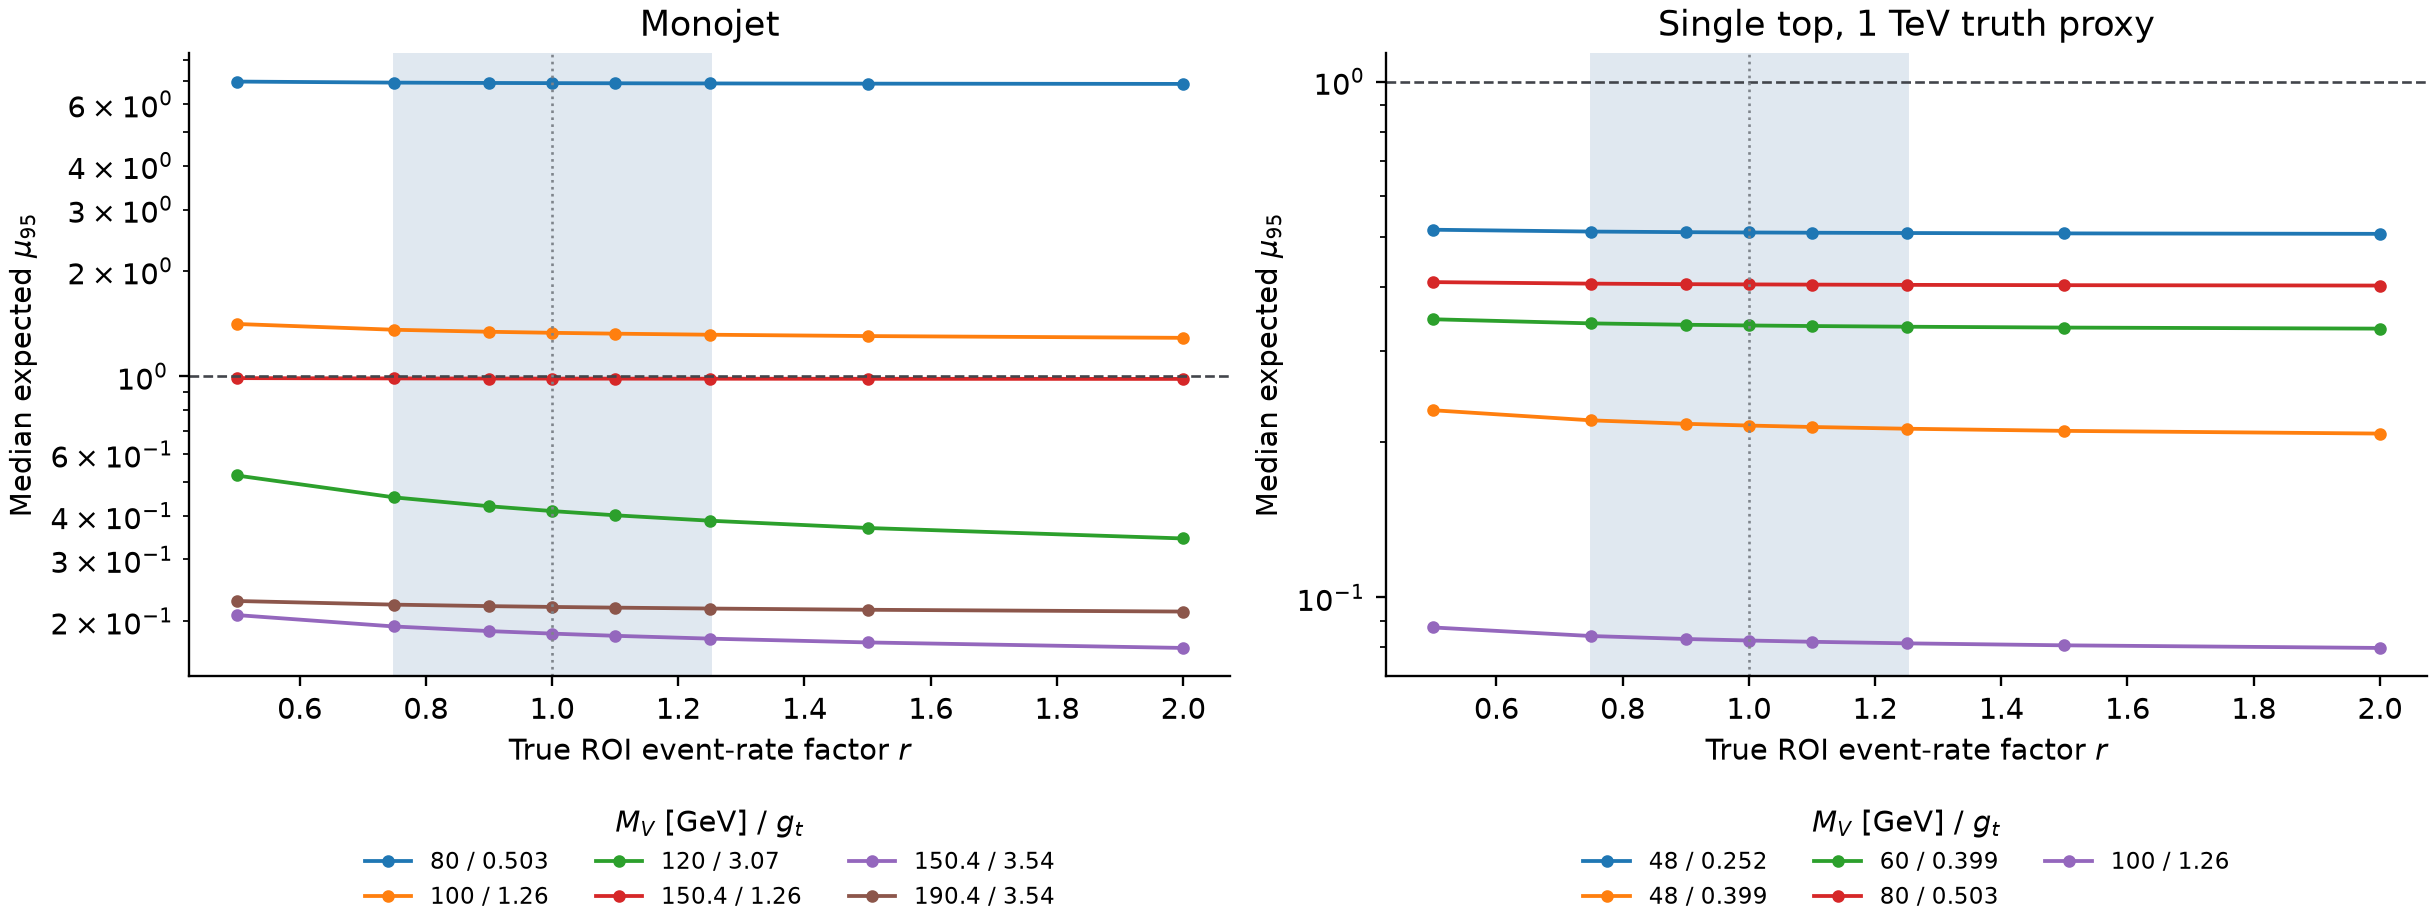
\includegraphics[width=.86\linewidth]{figures/07_lz_rate_variation.png}
\caption{We solve for the central Planck abundance and compute the CMS limit for each on-shell point at each fixed target yield. The shaded interval $r=0.75$--$1.25$ is the prescribed range for the normalization test, corresponding to $0.84$--$1.40$ expected truth-level events.}
\label{fig:rate}
\end{figure}

\section{Cross-section cuts and the mass projection}
\label{sec:production_checks}

The UFO for the closed quark loop includes a rational $R_2$ vertex for $gggV$ for each quark flavor. We replace the photon vector coupling in \texttt{loop\_sm} to obtain the coefficient $i g_{Vq}g_s^3/(48\pi^2)$ per flavor, with color structure $d^{abc}$. Including this term gives a numerical Ward/BRS test ratio of about $6.3\times10^{-24}$ for $gg\to gV$ at $M_V=87.18$ GeV and a partonic energy of 1 TeV. \cite{hirschi2015}

\begin{figure}[tbp]
\centering
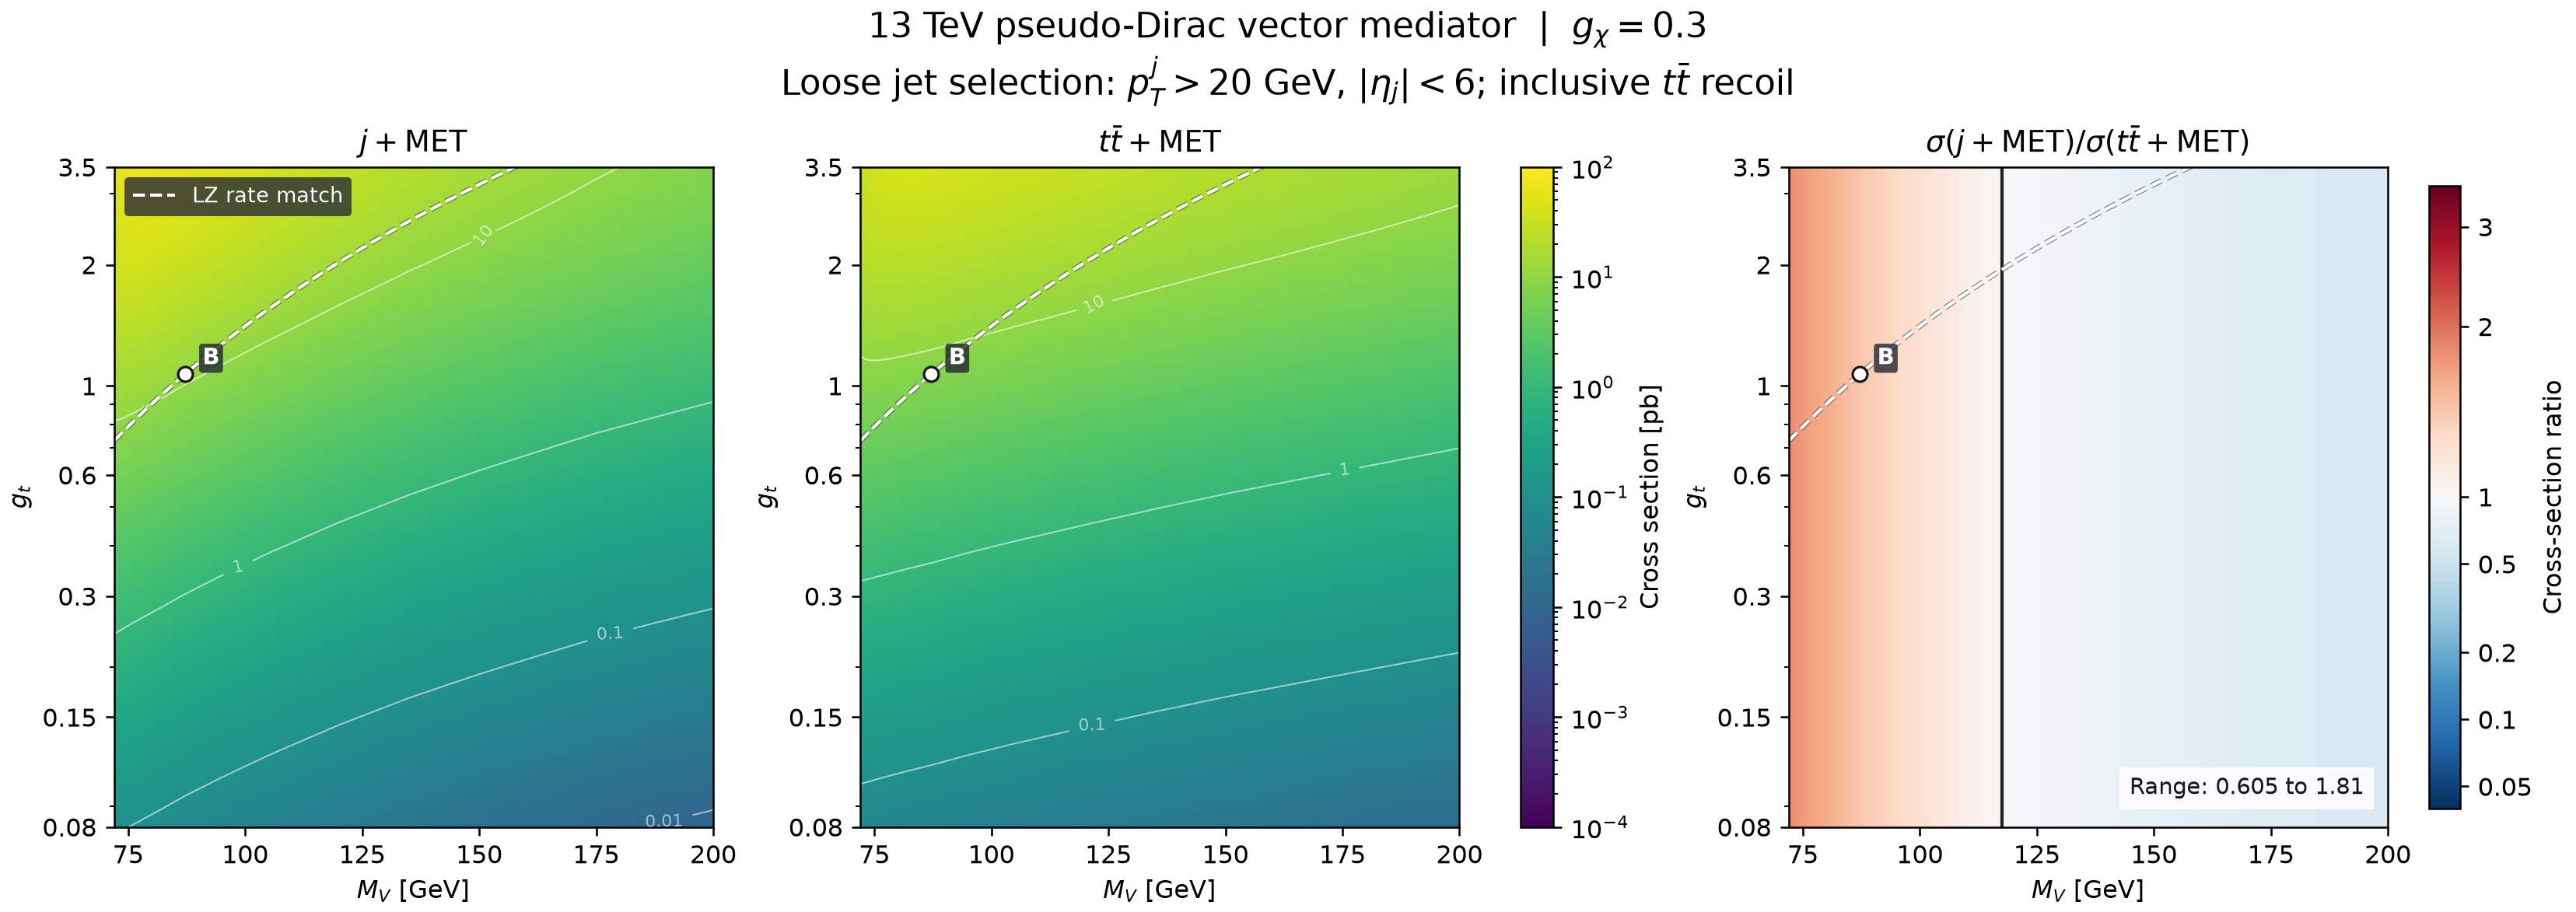
\includegraphics[width=.86\linewidth]{figures/b01_loose_cross_sections.png}
\caption{The jet selection is $p_T^j>20$ GeV and $|\eta_j|<6$, and the top-pair final state has no truth MET cut. Comparison with Fig.~\ref{fig:hard_met} shows the effect of the selection threshold.}
\label{fig:loose}
\end{figure}

\begin{figure}[tbp]
\centering
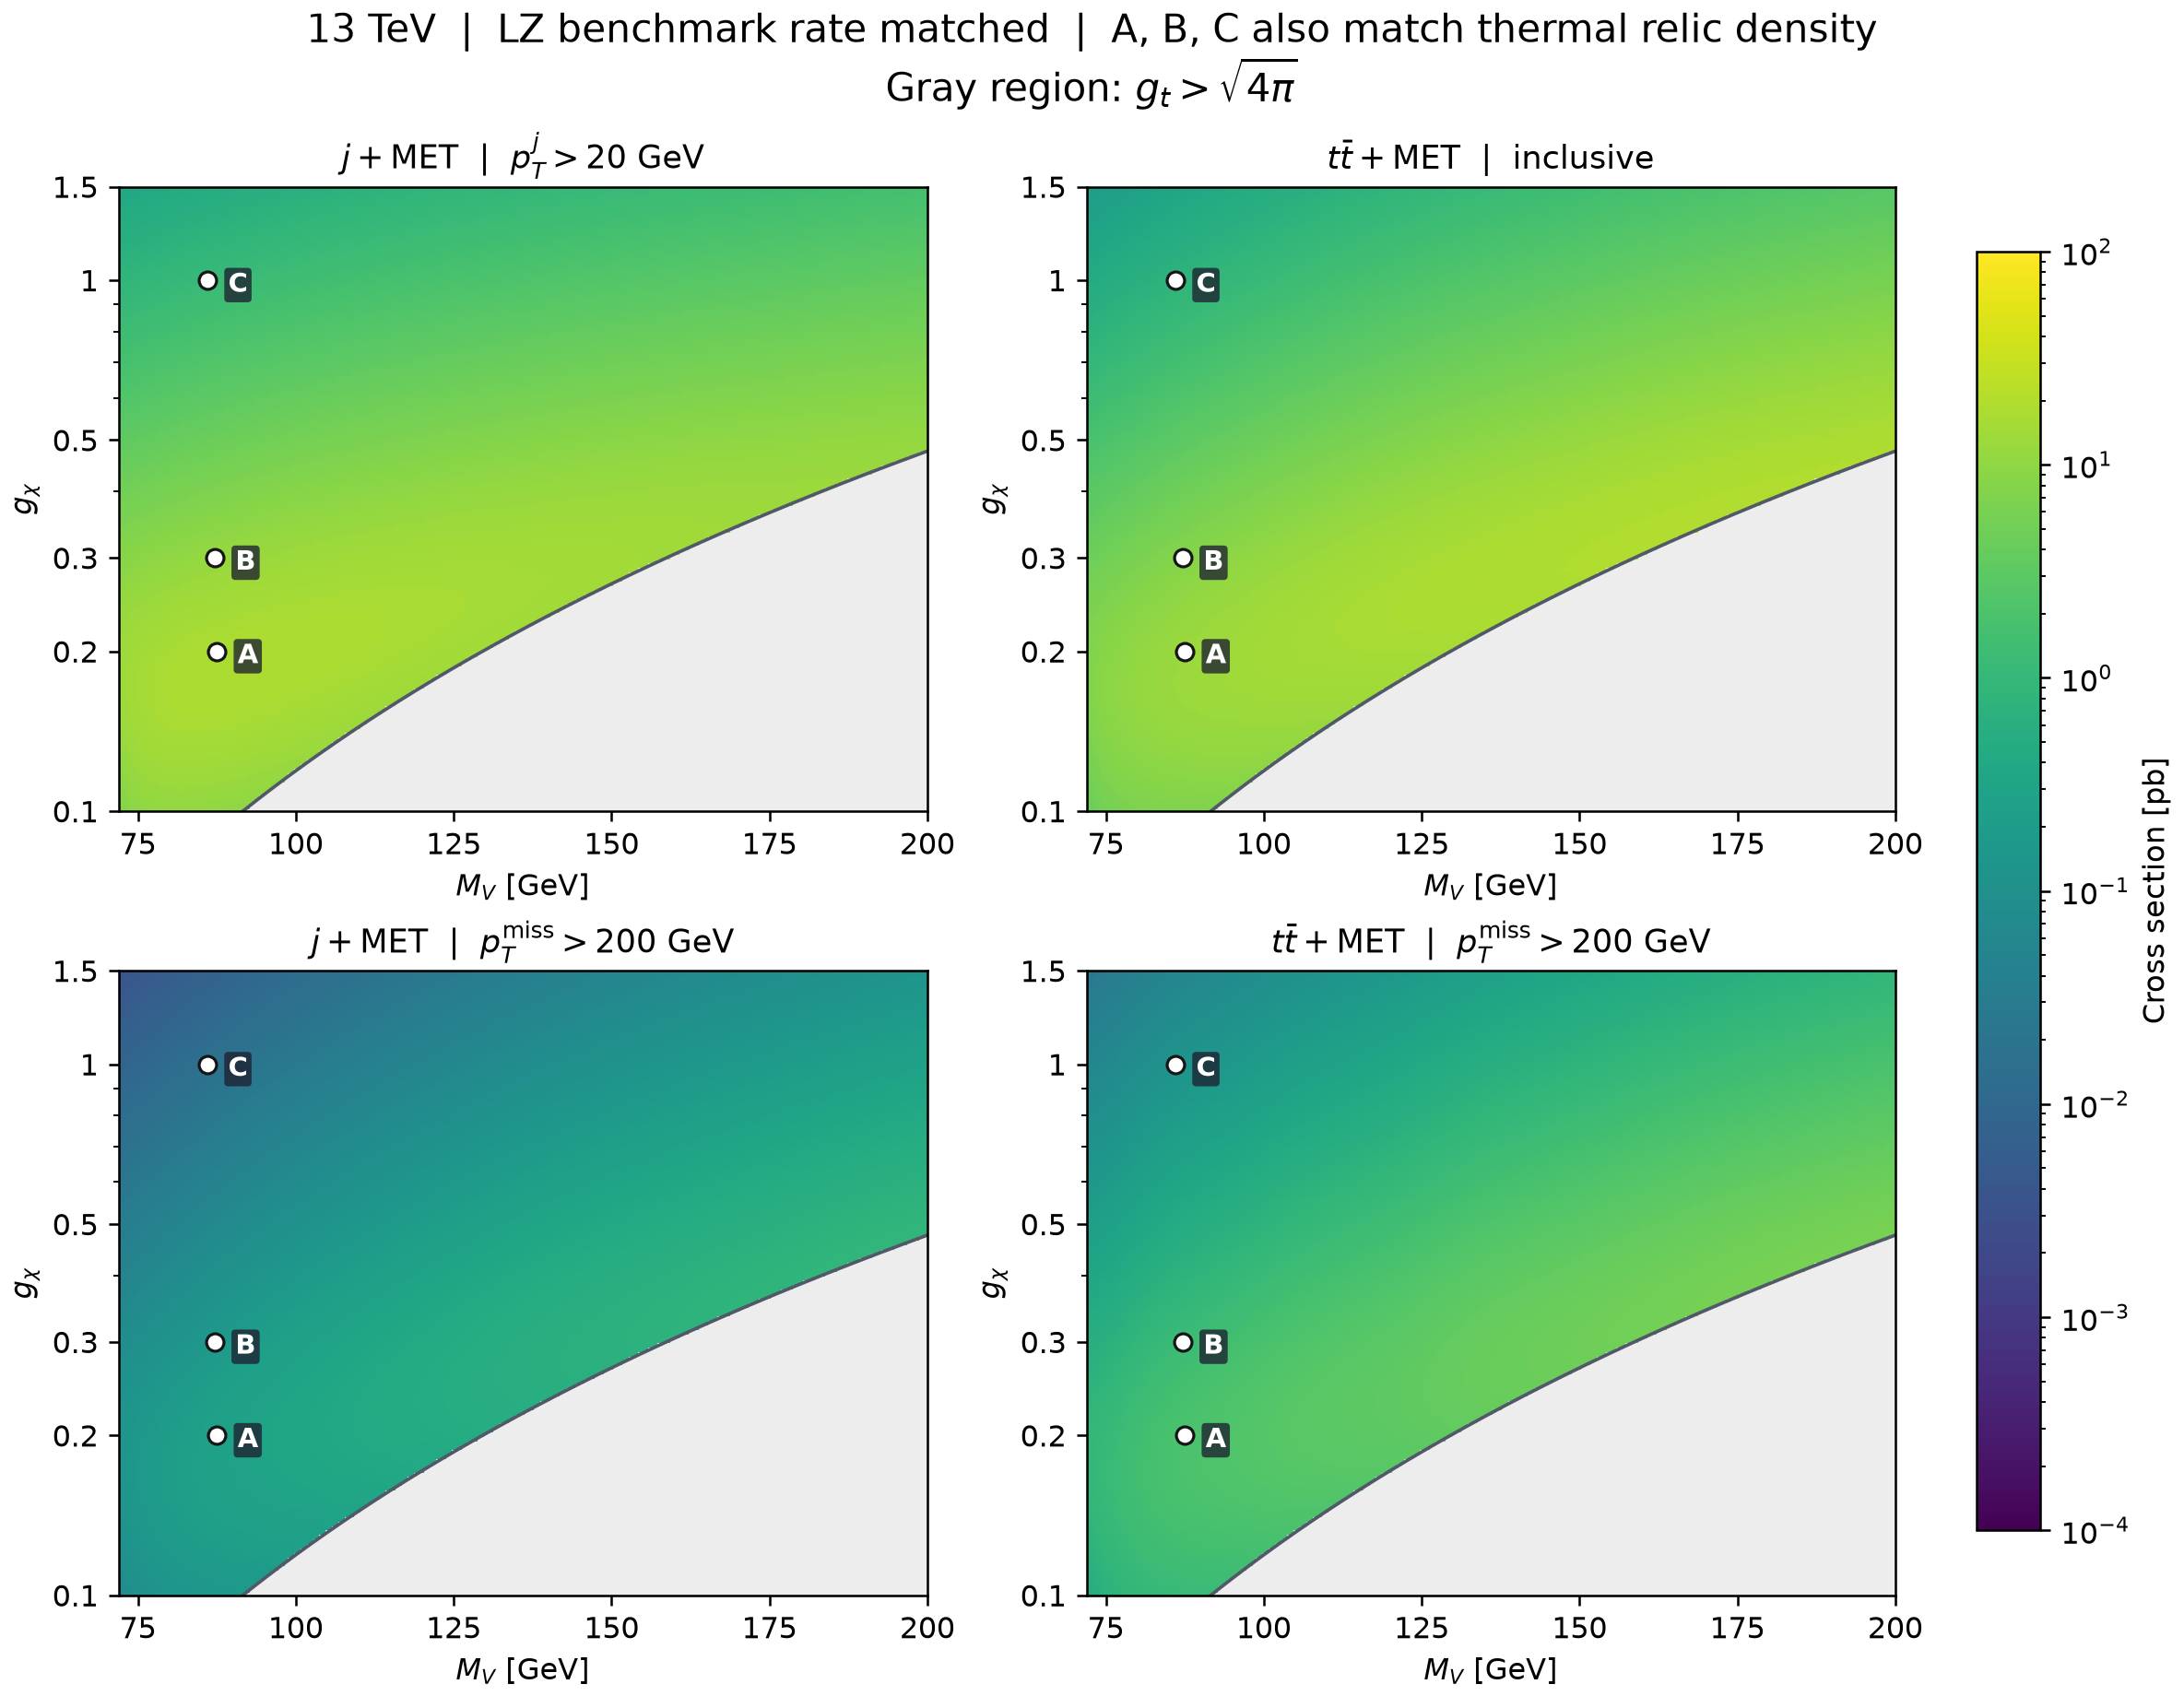
\includegraphics[width=.86\linewidth]{figures/b02_lz_slice_cross_sections.png}
\caption{We fix $m_\chi=35$ GeV and determine $g_t$ from the tree-level equal-rate condition. A, B, and C are separate relic-density benchmarks. The remaining colors show cross sections subject to the equal-rate condition alone.}
\label{fig:equal_rate_xsec}
\end{figure}

\begin{figure}[tbp]
\centering
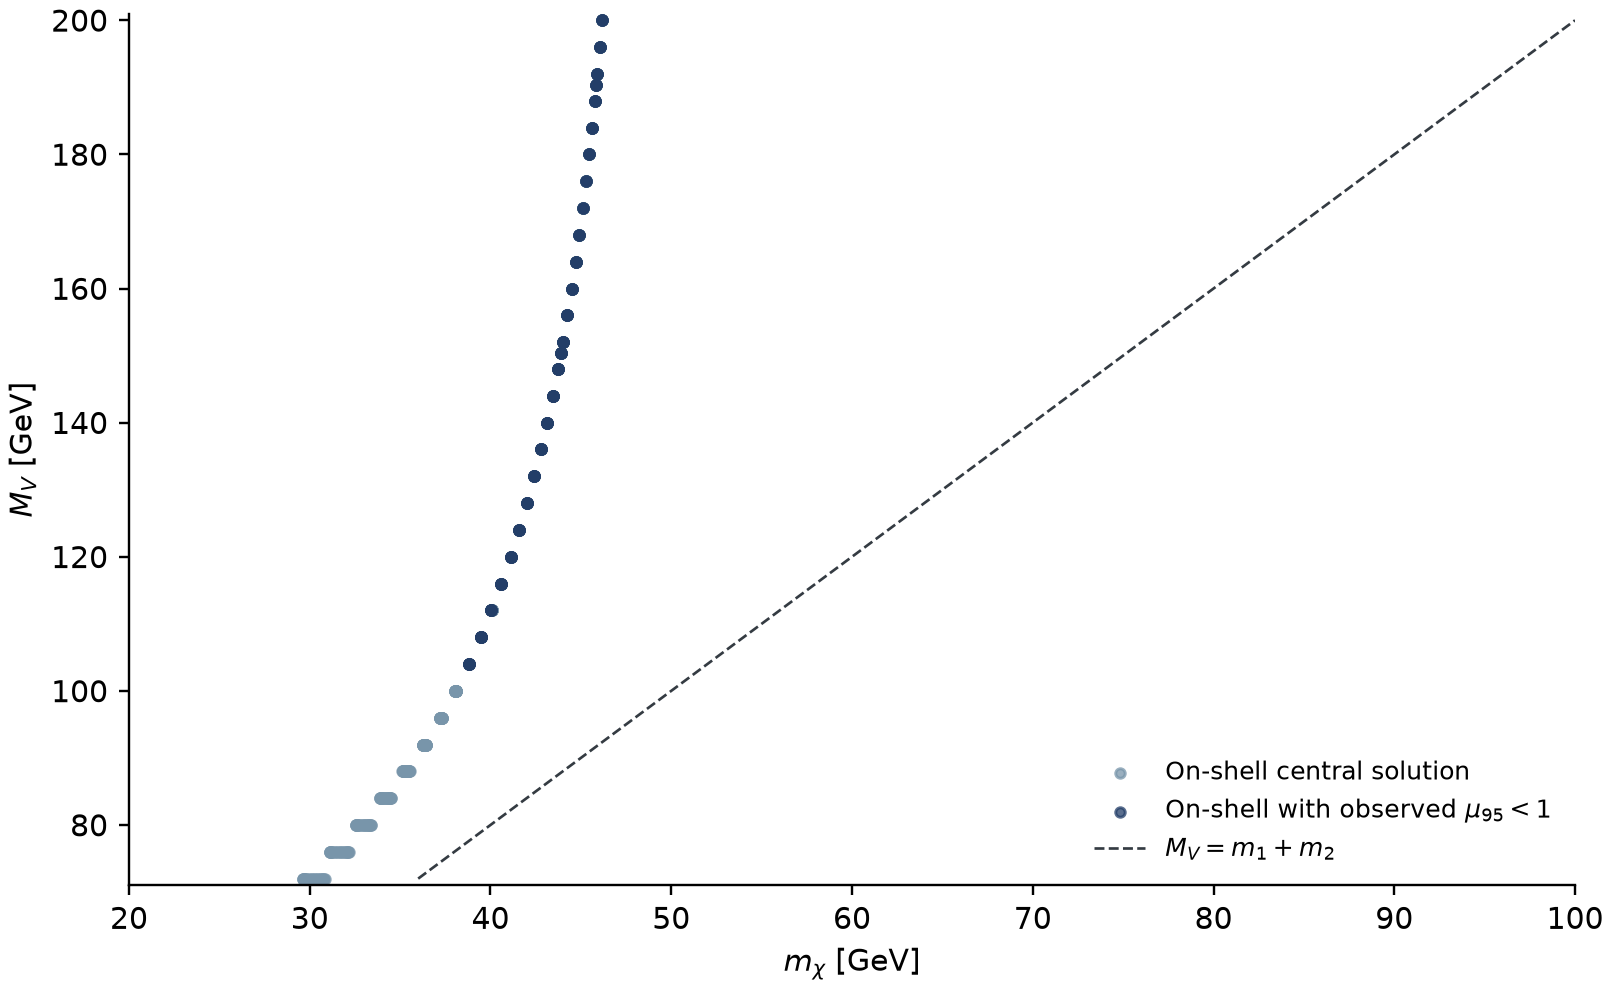
\includegraphics[width=.58\linewidth]{figures/04b_central_mass_projection.png}
\caption{Projection of the central relic grid onto $(m_\chi,M_V)$. Dark blue marks on-shell roots with observed $\mu_{95}<1$. Multiple coupling solutions can overlap in the mass projection.}
\label{fig:mass_projection}
\end{figure}

\section{Validation of the CMS monojet recast}
\label{sec:validation}

\begin{figure}[tbp]
\centering
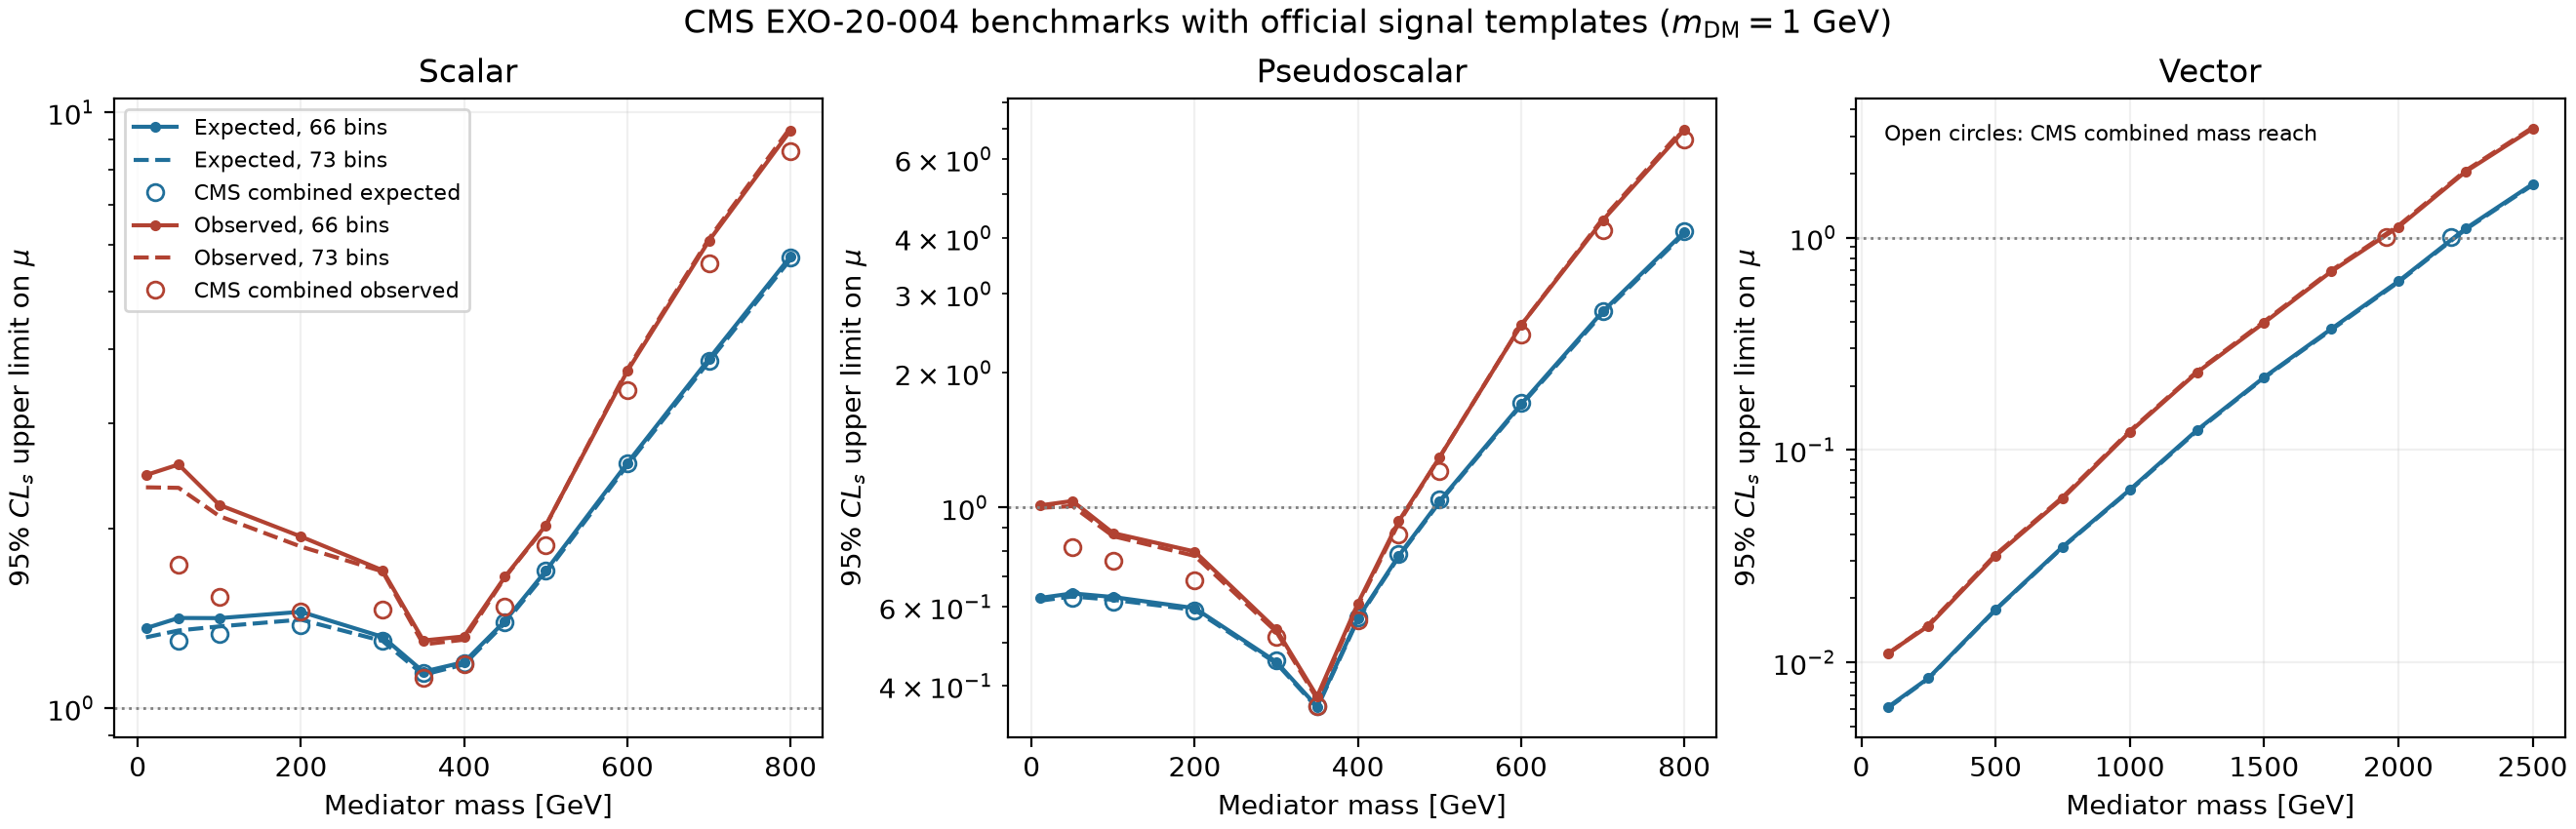
\includegraphics[width=.86\linewidth]{figures/c01_cms_benchmark_limits.png}
\caption{Comparison of limits obtained using official CMS signal templates. For scalar and pseudoscalar benchmarks between 50 and 800 GeV, the expected limits from the 66-bin fit differ from the published combination by at most about $9\%$. The largest difference in observed limits is about $48\%$. The mass boundaries provide a separate check of the overall reach for the official vector benchmark. \cite{cmsmonojet,cmssignal}}
\label{fig:cms_official}
\end{figure}

\begin{figure}[tbp]
\centering
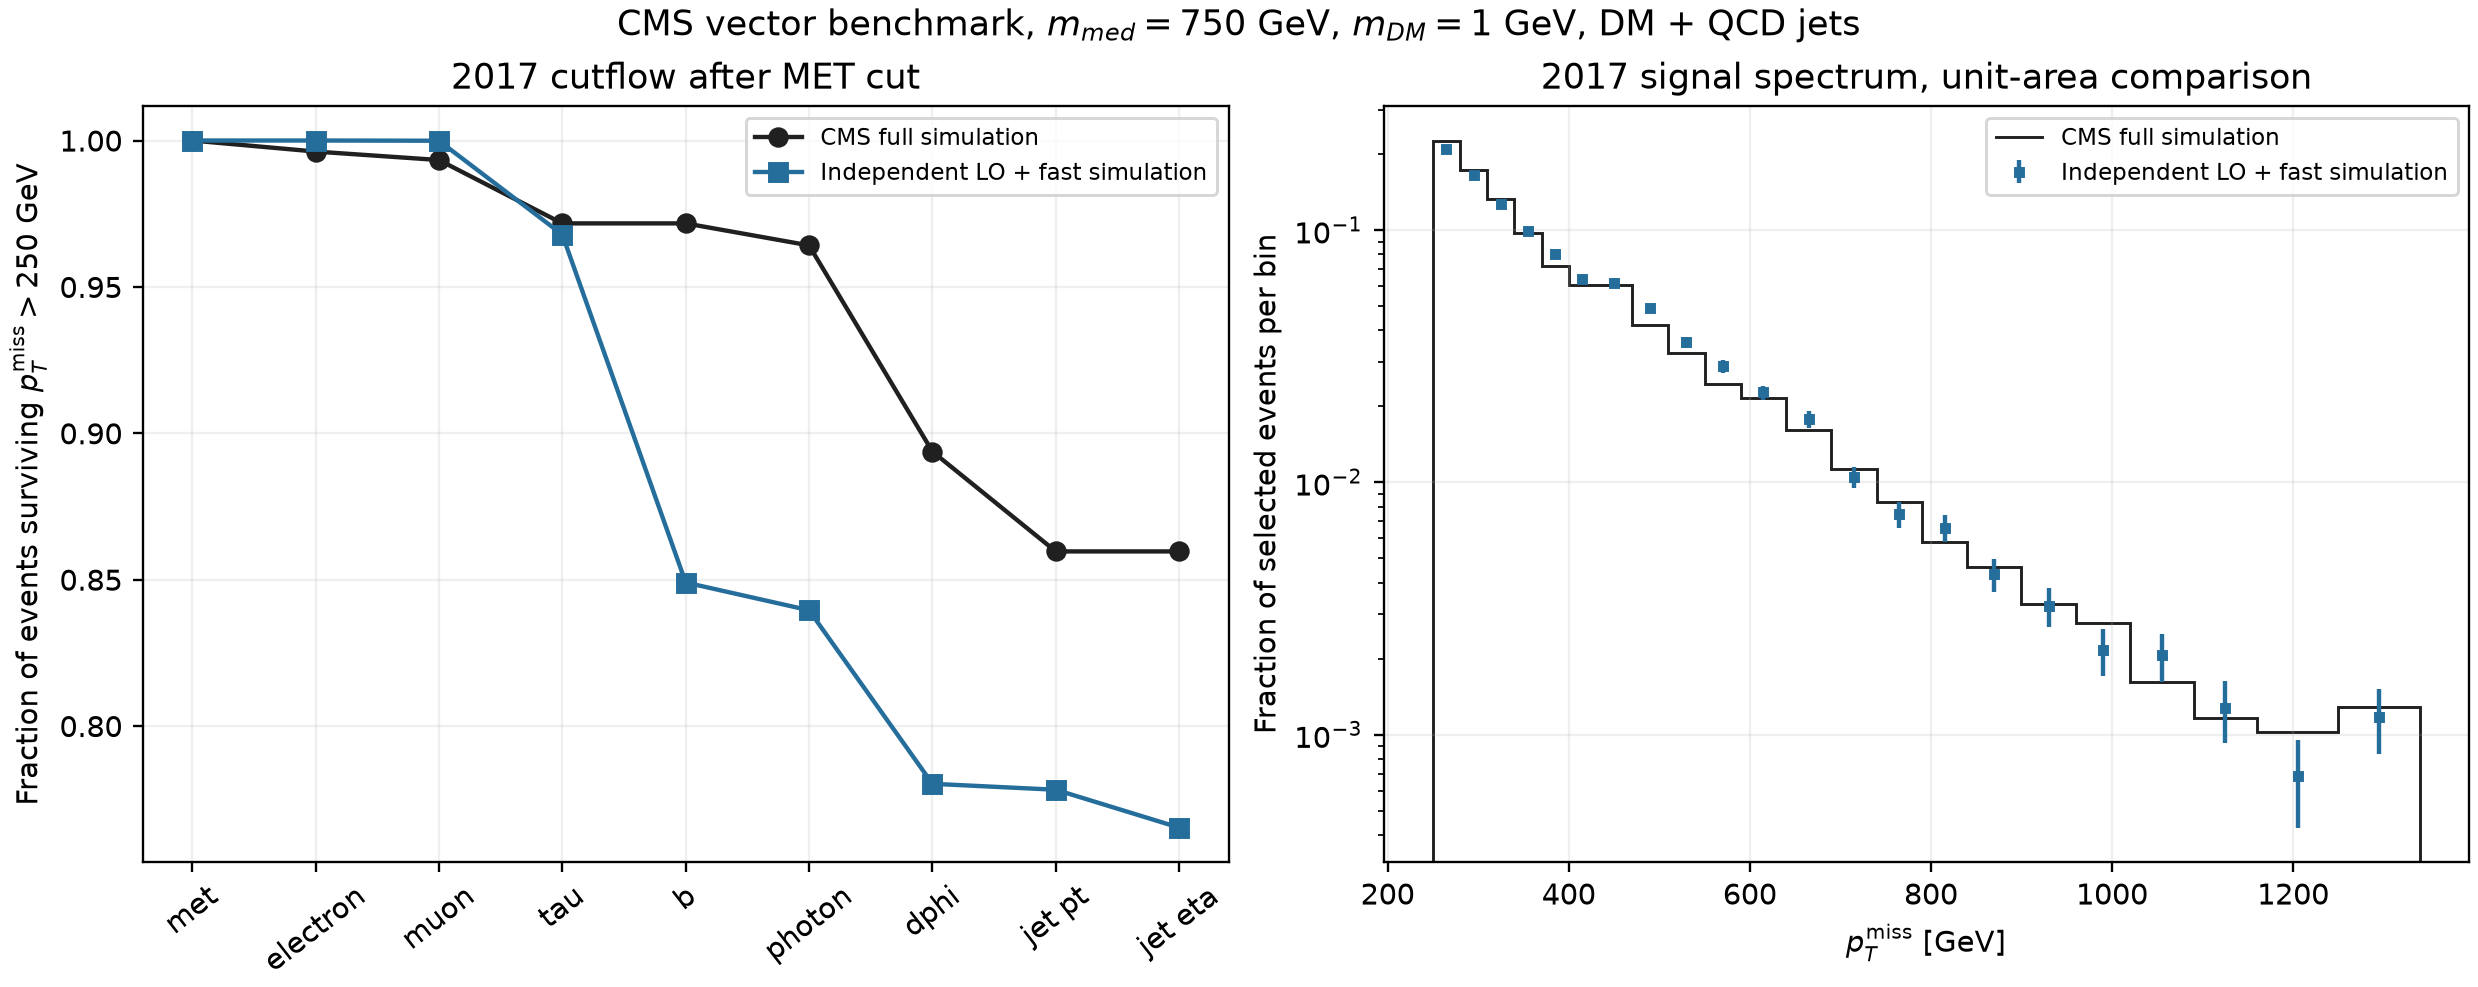
\includegraphics[width=.86\linewidth]{figures/c02_cms_vector_750.png}
\caption{Cutflow and MET spectrum for the 750 GeV CMS vector benchmark.}
\label{fig:cms_750}
\end{figure}

\begin{figure}[tbp]
\centering
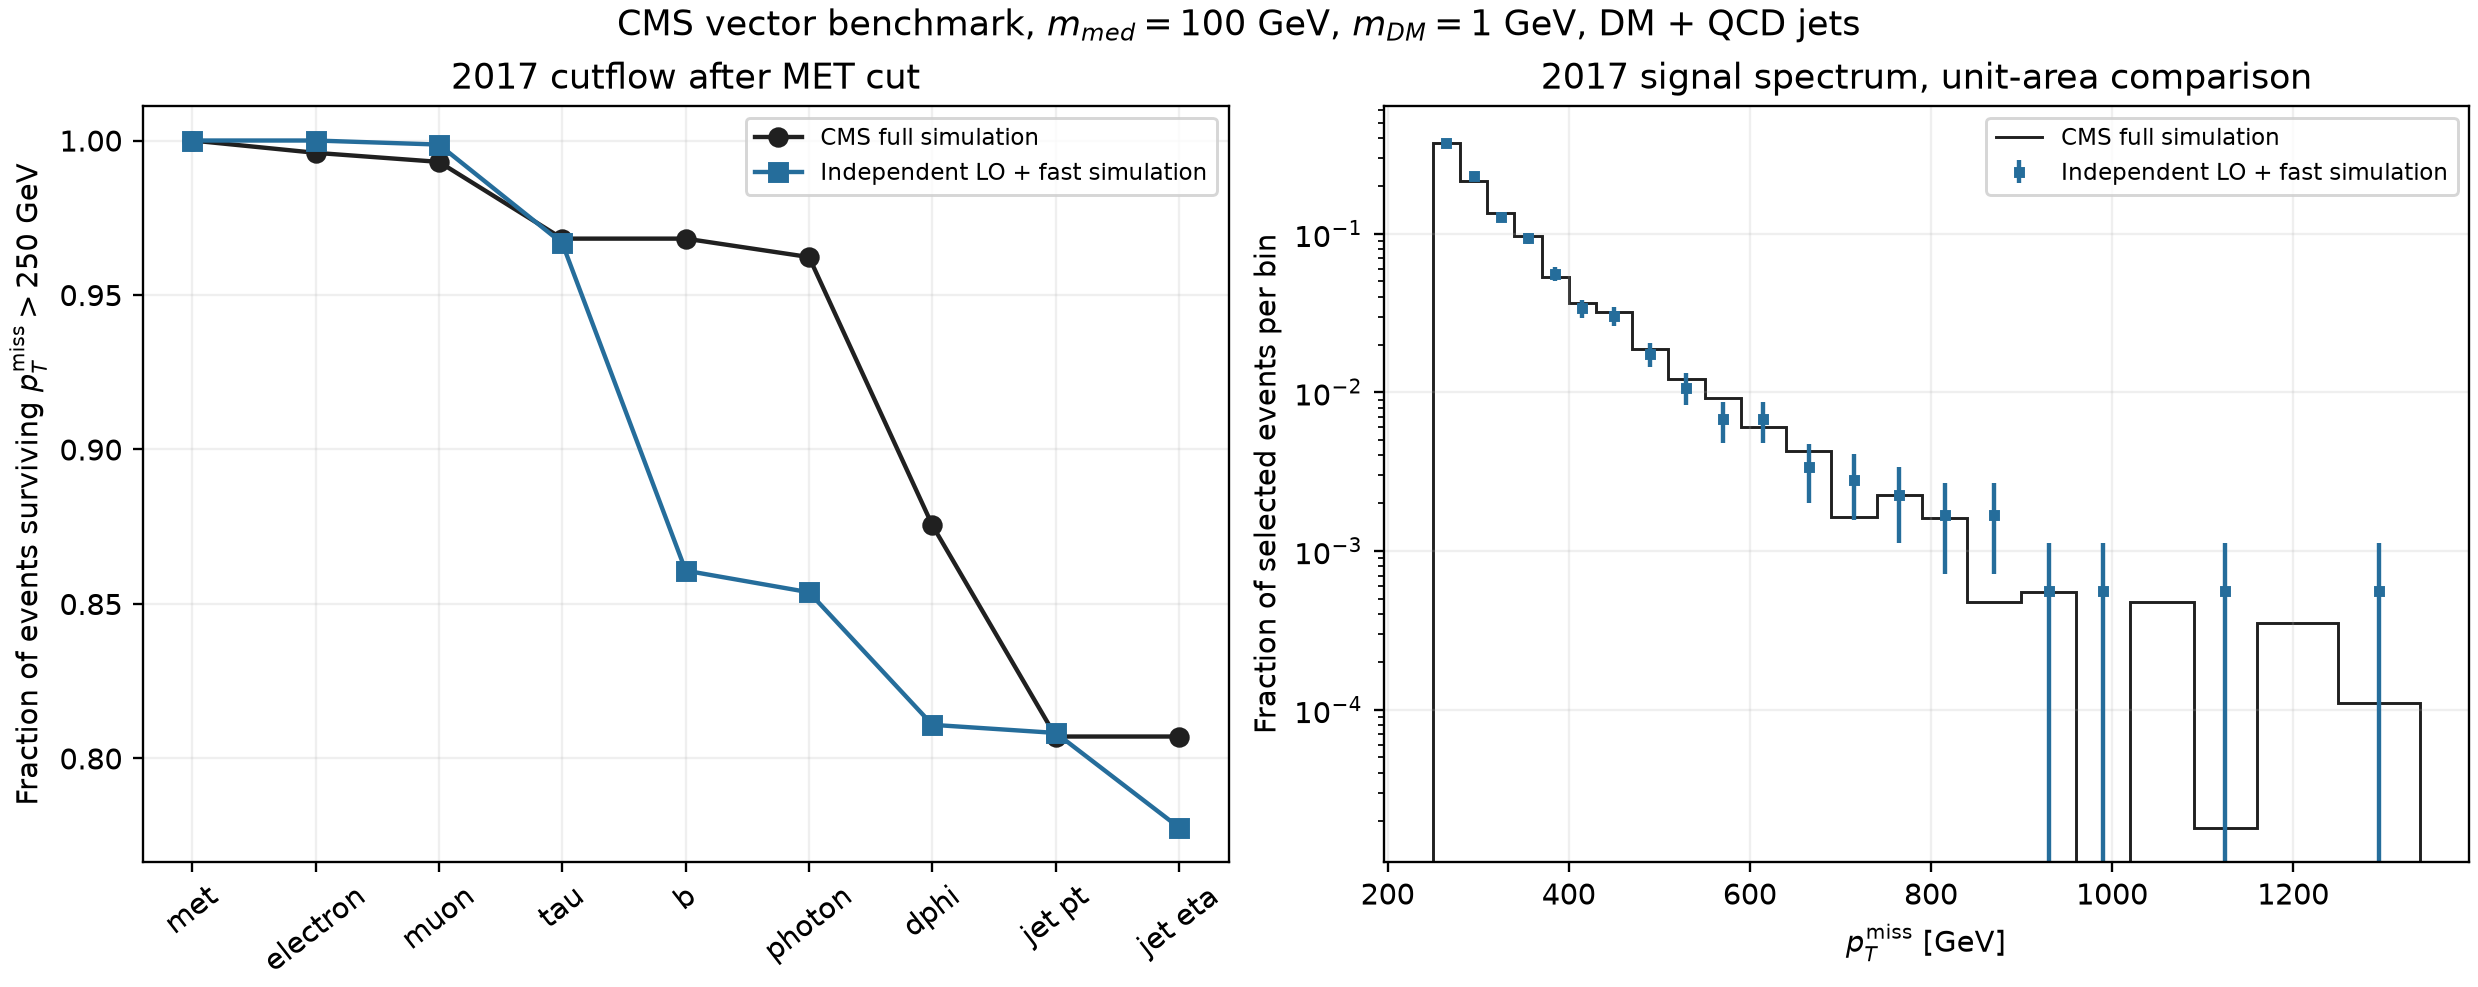
\includegraphics[width=.86\linewidth]{figures/c03_cms_vector_100.png}
\caption{Cutflow and MET spectrum for the 100 GeV CMS vector benchmark. Comparison of independent LO event generation and fast detector simulation with official CMS vector benchmarks. For the 100 GeV benchmark in 2017, the efficiency after the MET cut is $76.91\%$ for CMS and $77.76\%$ in our simulation. The absolute QCD signal yield in our simulation is 0.629 times the CMS yield. The two samples use different generator and reconstruction settings, including NLO matching in the official sample. We compare the normalized shapes and the absolute yields separately. \cite{cmscutflow}}
\label{fig:cms_100}
\end{figure}

\begin{figure}[tbp]
\centering
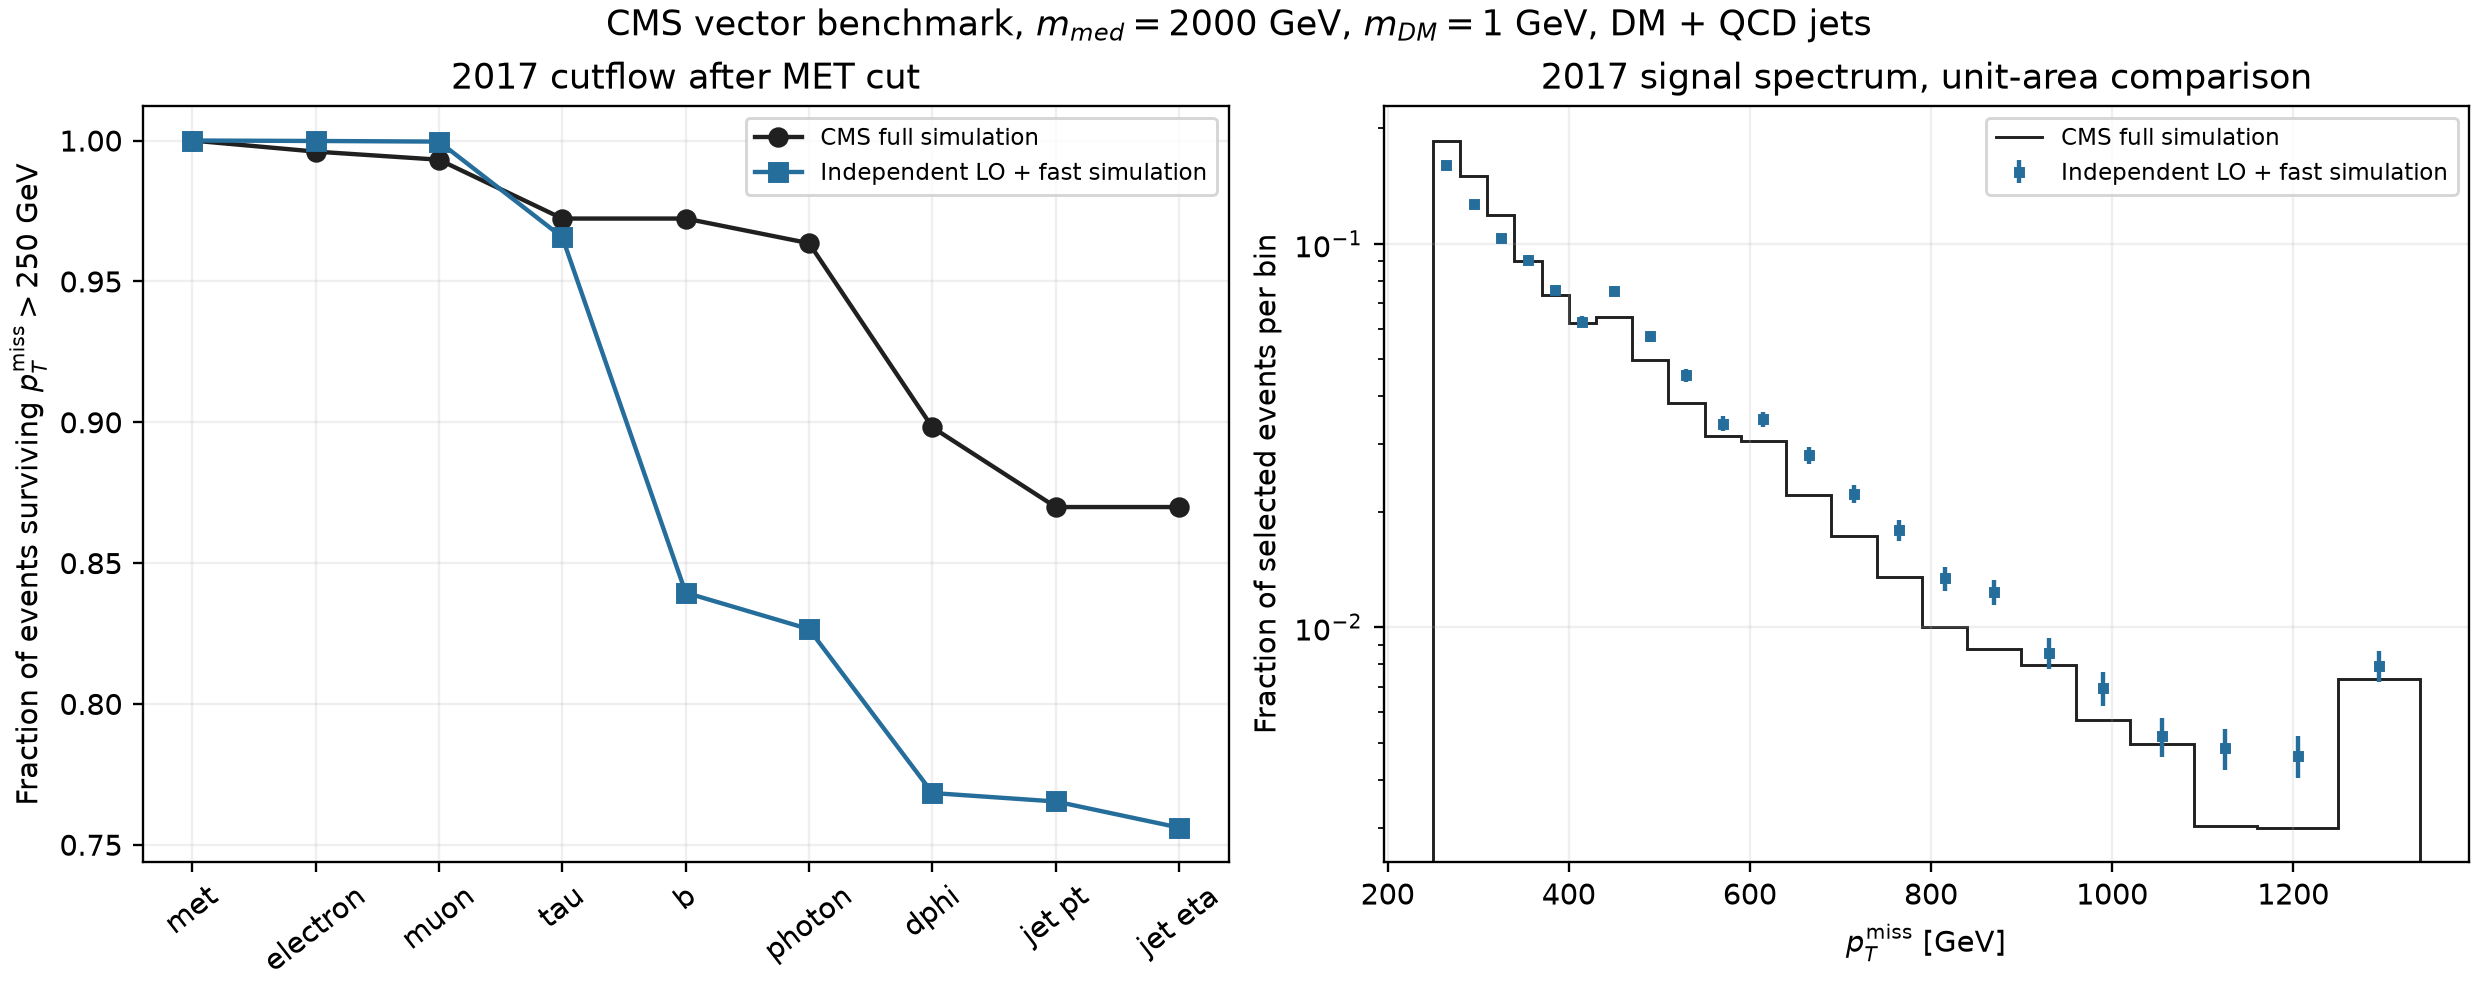
\includegraphics[width=.86\linewidth]{figures/c04_cms_vector_2000.png}
\caption{Cutflow and MET spectrum for the 2000 GeV CMS vector benchmark.}
\label{fig:cms_2000}
\end{figure}

\begin{figure}[tbp]
\centering
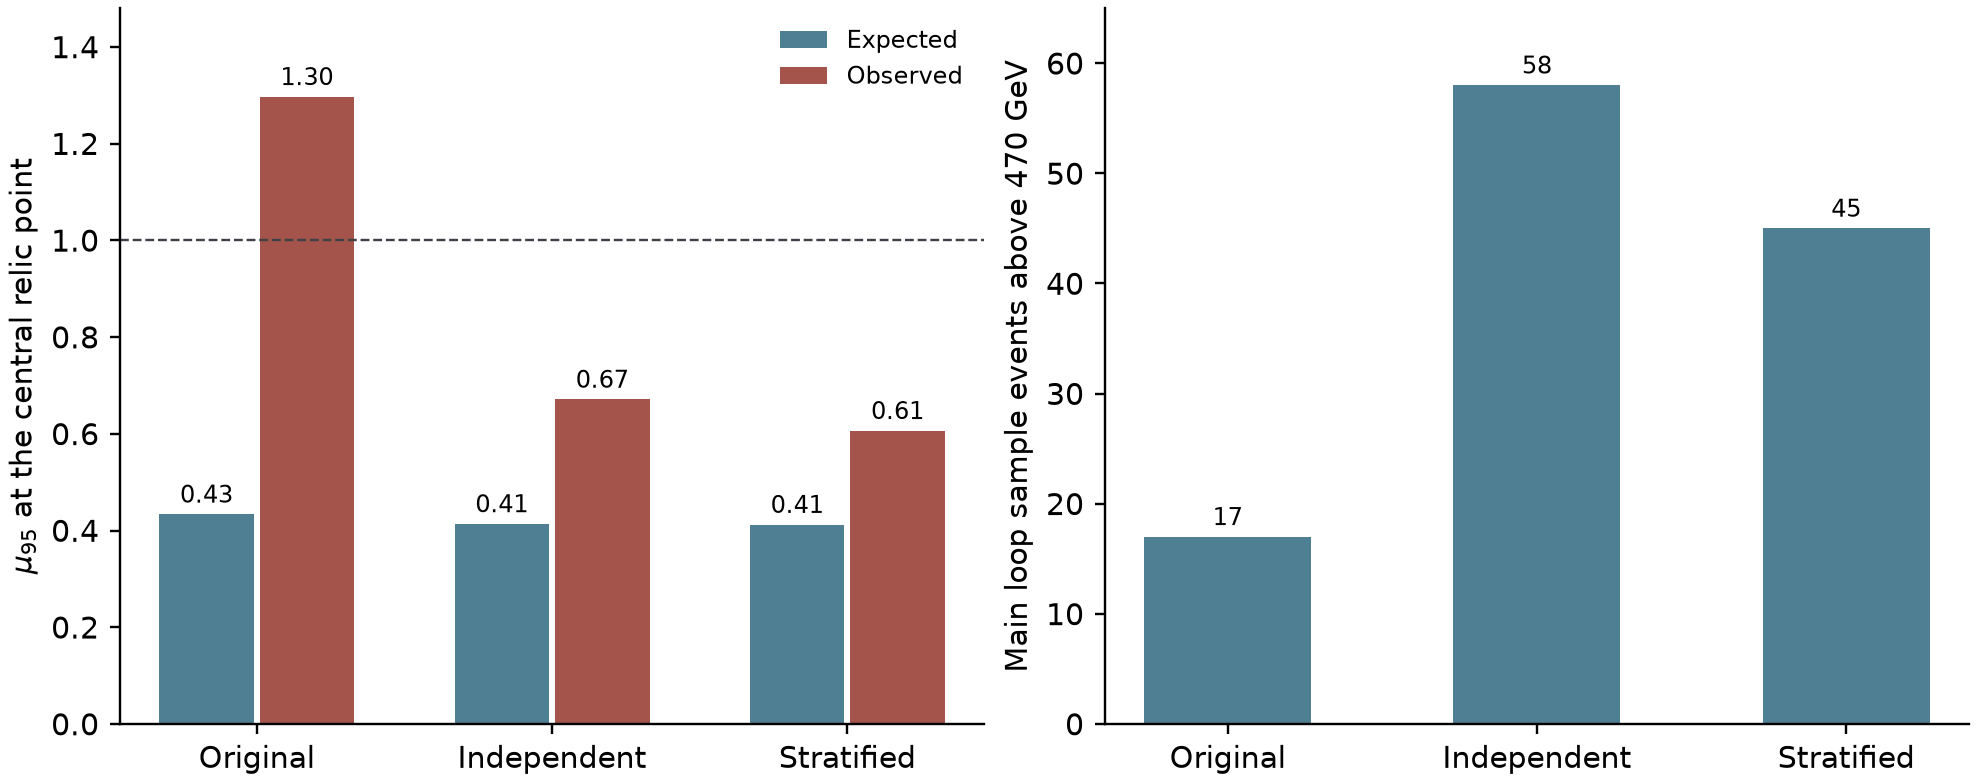
\includegraphics[width=.58\linewidth]{figures/c05_loop_mc_validation.png}
\caption{Of the 3,600 events in the original loop sample, 17 pass the reconstructed selection and fall in MET bins above 470 GeV. At the same central relic solution, the original sample gives an observed $\mu_{95}$ of about 1.30. An independent sample gives 0.67, and a stratified sample gives 0.61. The main analysis uses the stratified template and all observed counts.}
\label{fig:small_sample}
\end{figure}

\subsection{Independent template test at three sensitive benchmarks}

We keep $(M_V,g_t,m_\chi,g_\chi)$ fixed at the 120, 150.4, and 190.4 GeV benchmarks in Table~\ref{tab:benchmarks}, along with the 66-bin CMS likelihood and background covariance. Loop templates A and B use independent hard-process and shower samples, with generator-level jet $p_T$ boundaries of $(100,230,480)$ and $(100,260,520)$ GeV, respectively. The three strata typically contain 6,600, 4,000, and 3,200 generated events. For the lowest stratum of A at 120 and 150.4 GeV, we use an independent archived sample of 10,800 events and a new sample of 4,800 events, respectively, and retain events with $100\le p_T^j<230$ GeV. Both fits share a newly generated tree template. We also repeat both fits with the original tree template. We average the loop templates with equal weights, combine the Monte Carlo covariances with squared weights, and count the common tree uncertainty once.

We rank the year-specific MET bins using $|s_i[(C_b+\operatorname{diag}\mathbf b)^{-1}\mathbf s]_i|$, evaluated with the reference signal and the background-only information. In the eight highest-ranked bins, we compare the yield differences with the Monte Carlo uncertainties of the independent loop samples. We also sum yields across years in the 470--690 GeV and above-690 GeV intervals and refit the upper limits using all 66 bins.

\begin{table}[tbp]
\caption{Comparison of independent signal templates for the three sensitive benchmarks. The final column gives the largest discrepancy in one of the eight key bins in units of the Monte Carlo (MC) uncertainty.}
\label{tab:templates}
\begin{ruledtabular}
\begin{tabular}{rccc}
$M_V$ [GeV] & Expected A / B / pooled & Observed A / B / pooled & Max. difference ($\sigma_{\rm MC}$) \\
\hline
120 & 0.389 / 0.407 / 0.408 & 0.527 / 0.621 / 0.561 & 1.05 \\
150.4 & 0.230 / 0.243 / 0.242 & 0.219 / 0.254 / 0.234 & 0.88 \\
190.4 & 0.174 / 0.178 / 0.179 & 0.200 / 0.200 / 0.198 & 1.68 \\
\end{tabular}
\end{ruledtabular}
\end{table}

\begin{figure}[tbp]
\centering
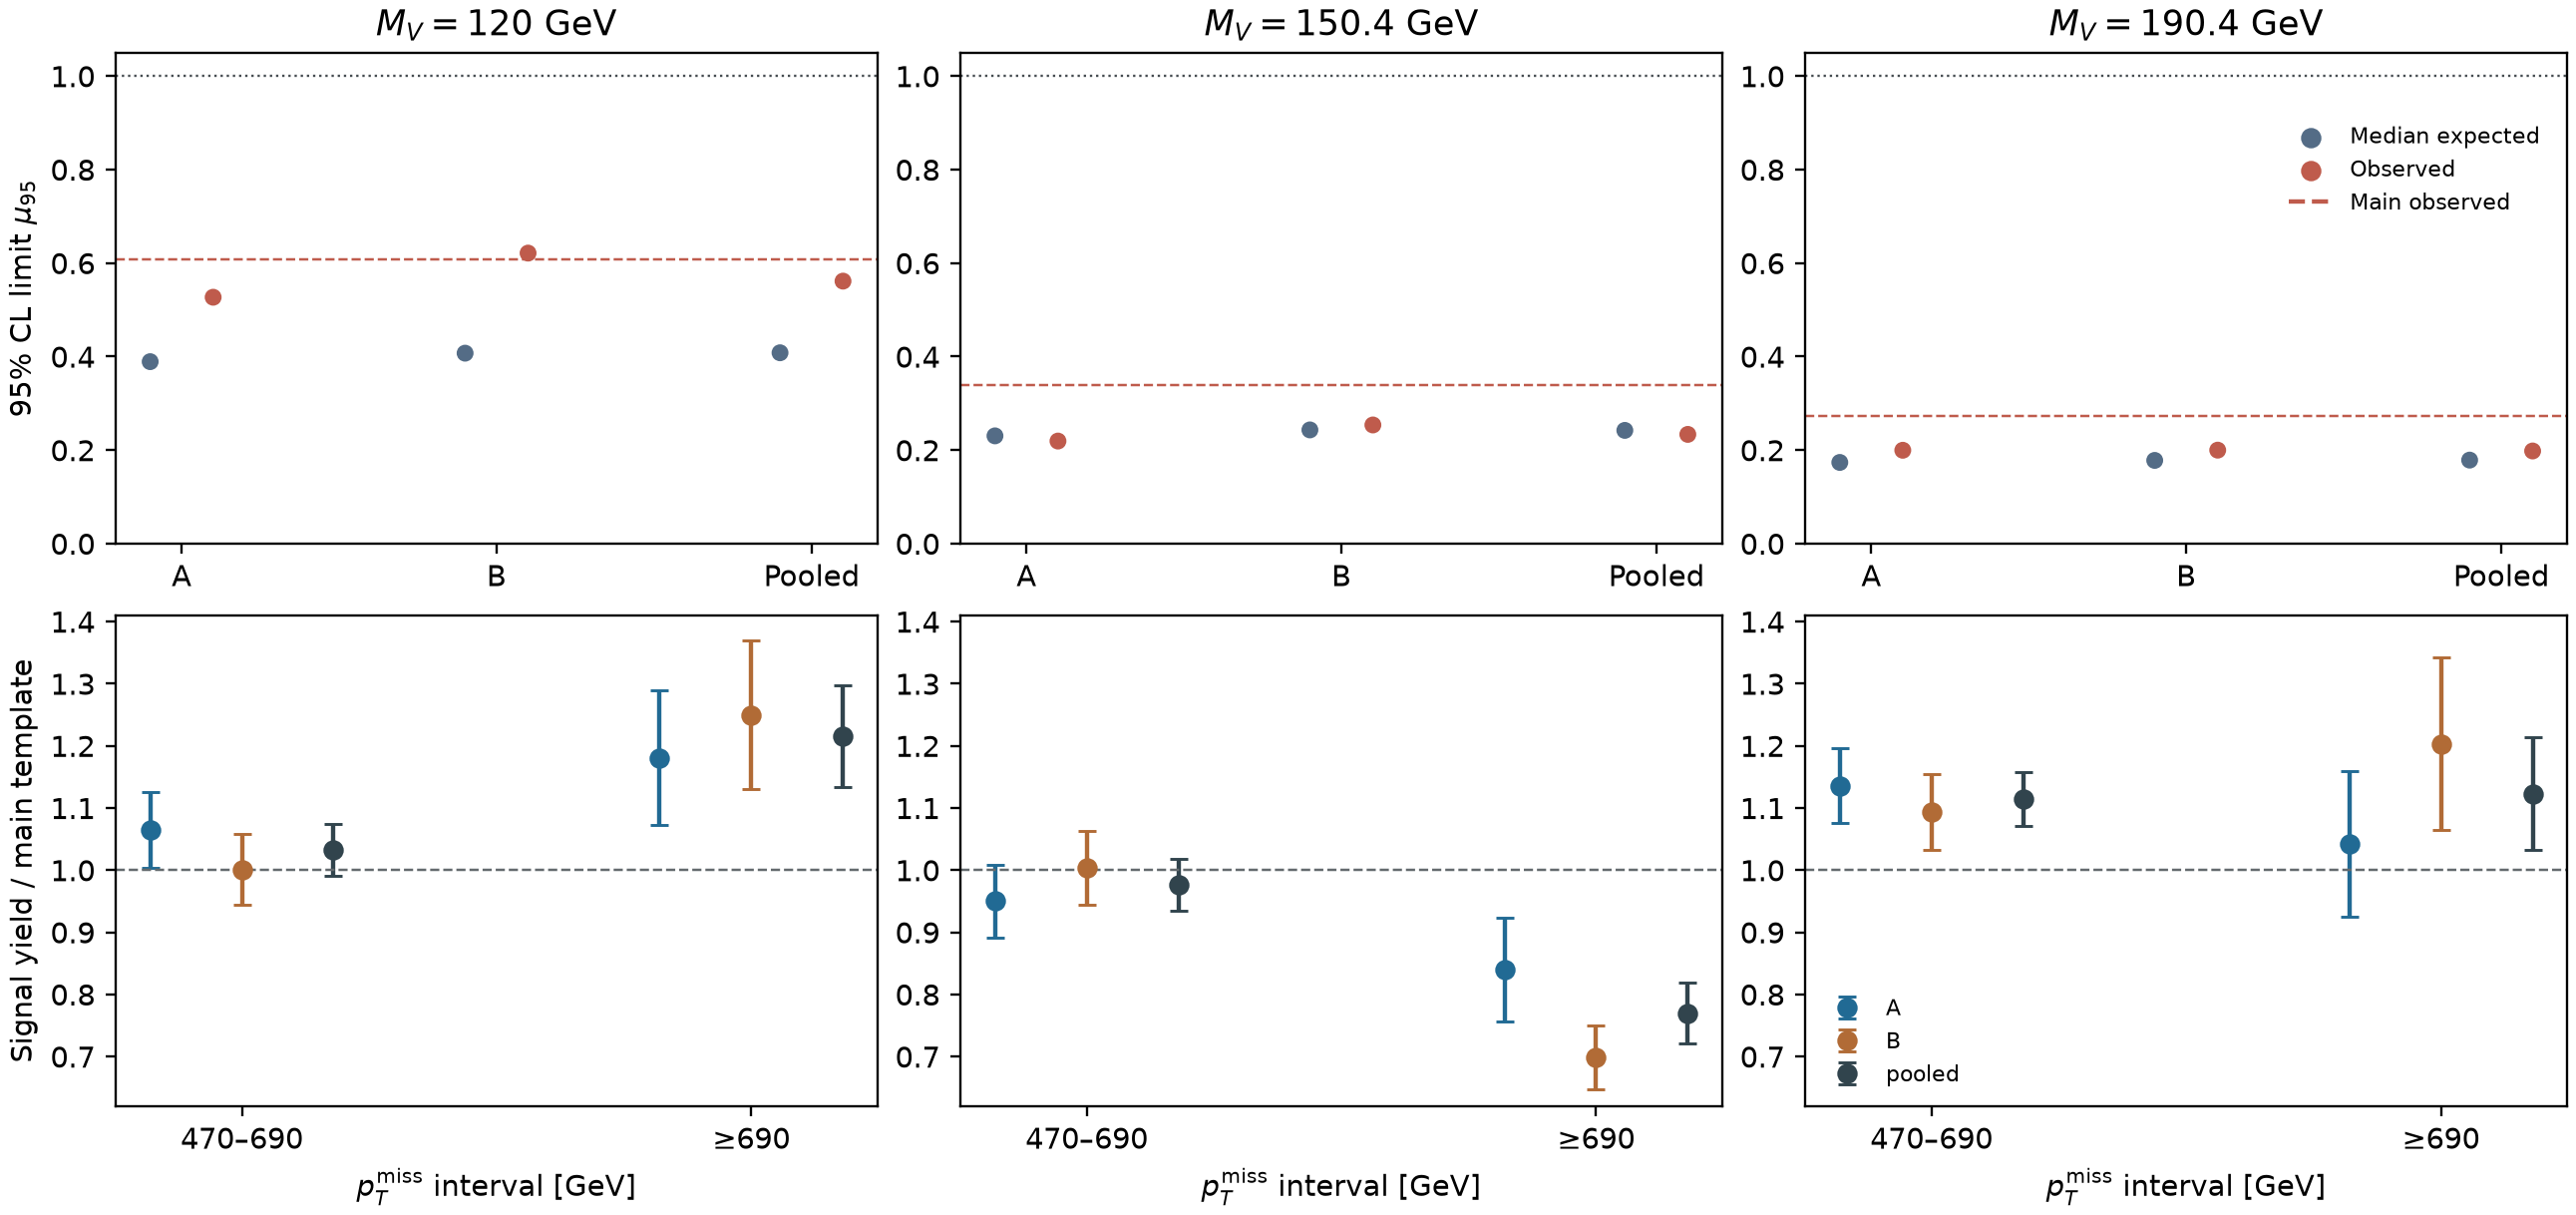
\includegraphics[width=.86\linewidth]{figures/c06_three_template_replicas.png}
\caption{The top panels show the CMS 95\% CL limits. The dashed lines mark the reference observed limits from Table~\ref{tab:benchmarks}. The lower panels show the yield of each template divided by the reference yield in two combined MET intervals. The error bars represent the Monte Carlo uncertainty of each template. The accompanying analysis tables give yields by year and bin.}
\label{fig:independent_samples}
\end{figure}

The two templates agree within about $1.7$ Monte Carlo standard deviations in the key bins and combined high-MET intervals. All three benchmarks give observed $\mu_{95}<1$. Across templates and target yields in the range $r=0.75$--$1.25$, the largest observed limit is $0.680$. At 120 and 150.4 GeV, the two stratifications still give observed limits that differ by about $16\%$ and $15\%$ of their mean, respectively. At 150.4 and 190.4 GeV, the pooled limits are about $31\%$ and $27\%$ below the reference values in Table~\ref{tab:benchmarks}. The three exclusion decisions are stable across the sampling schemes tested, while the numerical limits retain some dependence on Monte Carlo statistics and template shape.

We refit the original grid with the three pooled templates, replacing the 120 and 150 GeV nodes and adding the 190.4 GeV node. After interpolation, the number of points with expected $\mu_{95}<1$ changes from 208 to 199, and the observed count changes from 151 to 162. The lowest sampled masses remain 92 and 104 GeV, respectively. The absolute yield discrepancy in Fig.~\ref{fig:cms_100} still limits the validation of the signal acceptance.

\section{Top-associated channels for light mediators}
\label{sec:top}

\subsection{Top-pair production}

With the loose jet cut $p_T^j>20$ GeV, the truth-level $j+\mathrm{MET}$ cross section is comparable to the inclusive $t\bar t+\mathrm{MET}$ cross section near $M_V\simeq118$ GeV. Applying $p_T^{\rm miss}>200$ GeV to both channels gives a cross-section ratio $\sigma(j+\mathrm{MET})/\sigma(t\bar t+\mathrm{MET})$ of $0.135$--$0.149$. For example, at $(m_\chi,M_V,g_t,g_\chi)=(35,87.18,1.070,0.30)$ the two cross sections are $0.166$ and $1.23$ pb, respectively. We treat the top quarks as stable, so $p_T^{\rm miss}=p_T(V)$. \cite{cox2016,alwall2014,hirschi2015}

\begin{figure}[tbp]
\centering
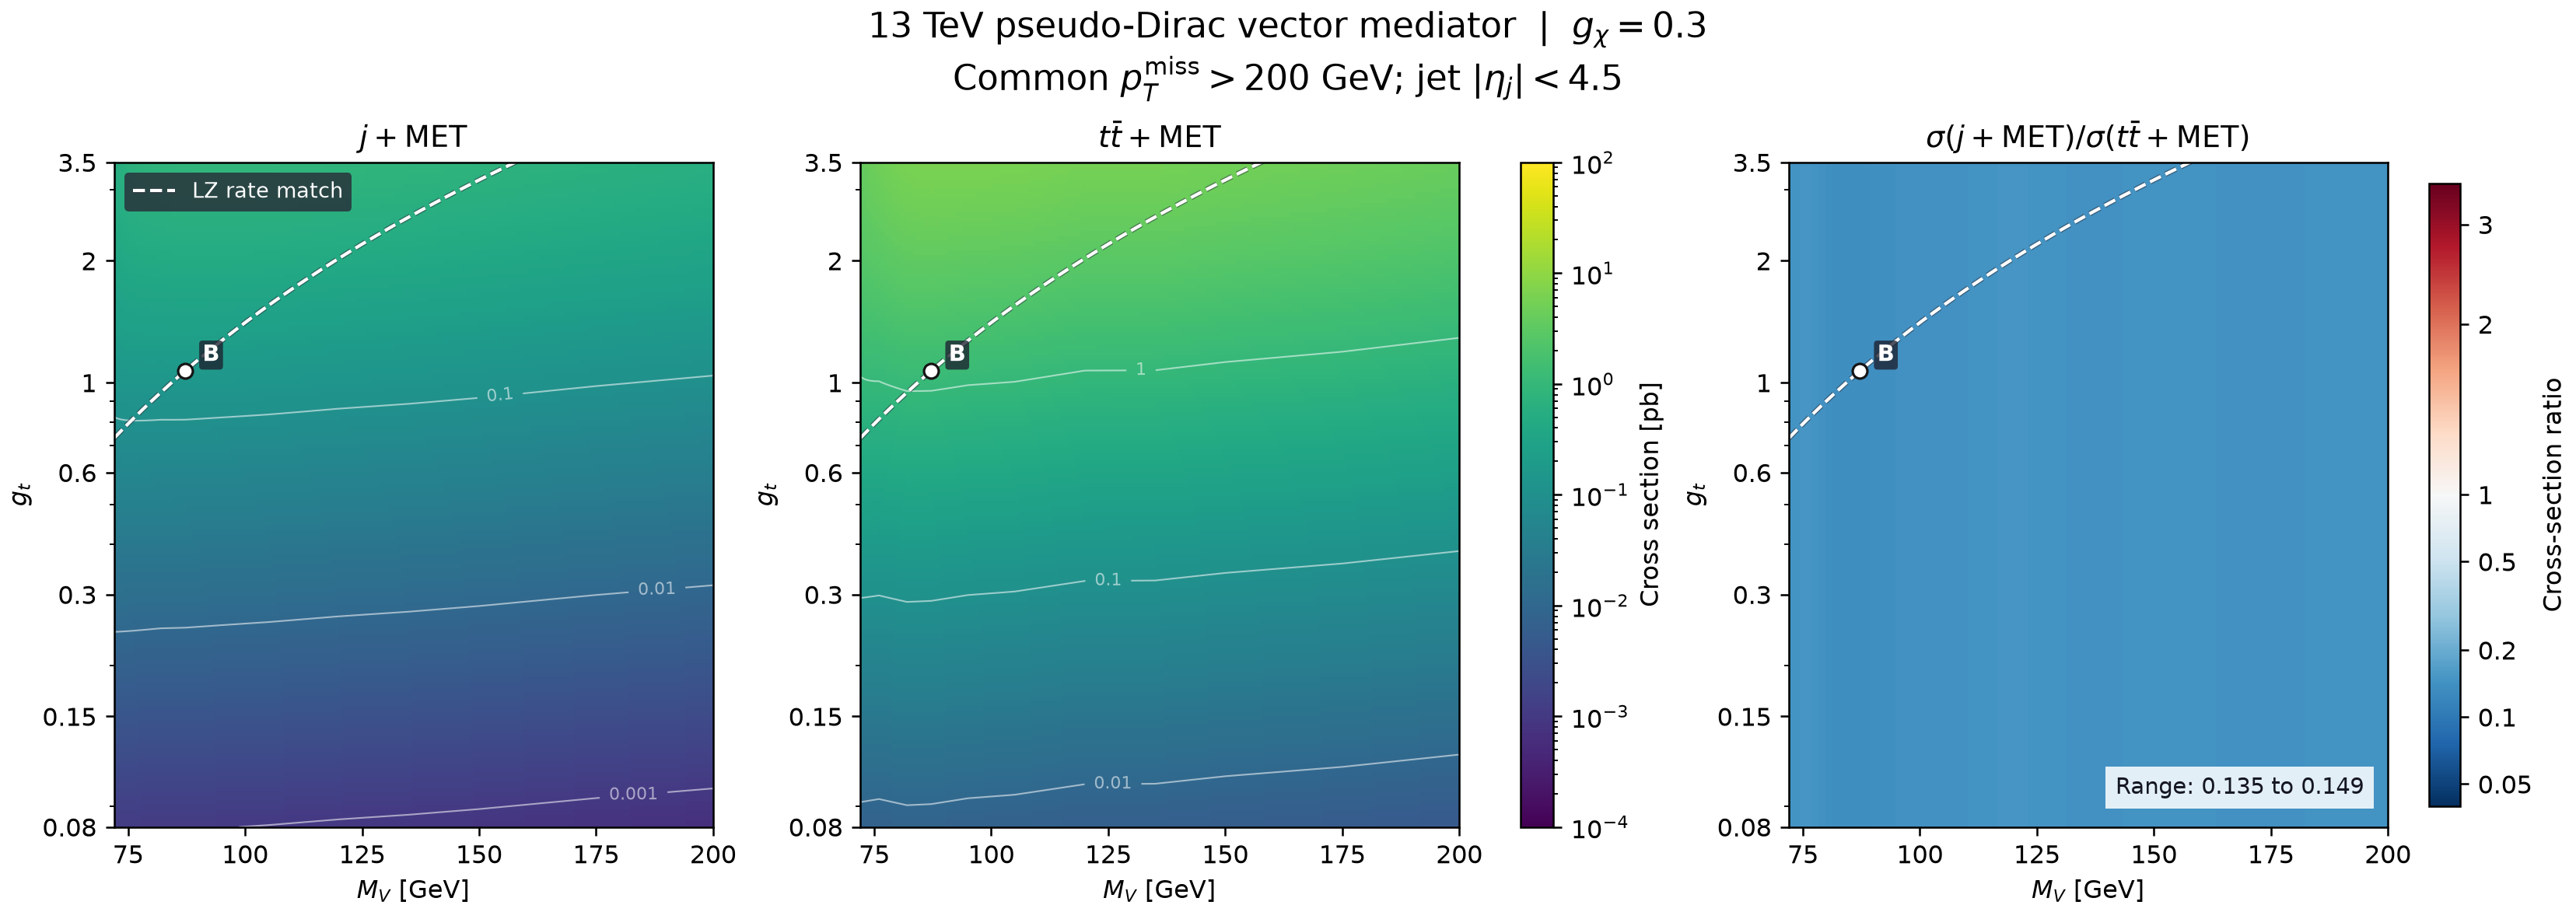
\includegraphics[width=.86\linewidth]{figures/03_hard_met_cross_sections.png}
\caption{Truth-level cross sections in pb and their ratio for $m_\chi=35$ GeV and $g_\chi=0.30$. The dashed curve shows the tree-level LZ yield-matching condition. The monojet cross section includes the leading tree channels and the $gg\to gV$ loop contribution.}
\label{fig:hard_met}
\end{figure}

The large top-quark coupling $g_t$ makes $pp\to t\bar tV^{(*)}\to t\bar t\chi_1\chi_2$ another possible collider probe. On-shell enhancement can occur when $M_V>2m_\chi+\Delta m$. Below this threshold we generate the four-body final state directly. In the low-mass scan, $(M_V,g_t)=(48\,\mathrm{GeV},0.252)$ has three solutions at the central abundance, with $m_\chi=20.445,25.260,45.878$ GeV. The lightest solution is on shell. At off-shell benchmarks with $M_V=30,46,60$ GeV, the full matrix element at 13 TeV gives $t\bar t+\mathrm{MET}$ cross sections of $0.033$, $0.041$, and $1.13$ fb, respectively, for truth-level $p_T^{\rm miss}>250$ GeV. Limits in the CMS all-hadronic two-$b$-tag category also require the acceptance after top decays, the binned signal yields, and the background correlations. \cite{cmstop}

\subsection{Single-top sensitivity}

For the single-top channel $pp\to tj\chi_1\chi_2$, we estimate the expected sensitivity in the 15 bins of the CMS AH $1b\,1\mathrm{FJ}$ category. We approximate the backgrounds with the published central values and bin uncertainties from the fit with a 100 GeV scalar signal, keeping only the diagonal covariance. For the signal we use truth-level cuts, simplified top decays, and approximate $b$ tagging. At $(M_V,g_t)=(60\,\mathrm{GeV},0.399)$, the cuts $\sqrt{\hat s}<1.5,1.0,0.75$ TeV give median expected limits of $0.052,0.337,3.43$, respectively. The strong dependence on this cut is related to the charged weak current connecting up- and down-type quarks with unequal vector couplings. We use the cut variation to test the contribution of high-energy events. A quantitative exclusion requires an electroweak completion and validation of the reconstructed signal and background constraints. \cite{kahlhoefer2016,cmstop,cmsahdata}

\begin{figure}[tbp]
\centering
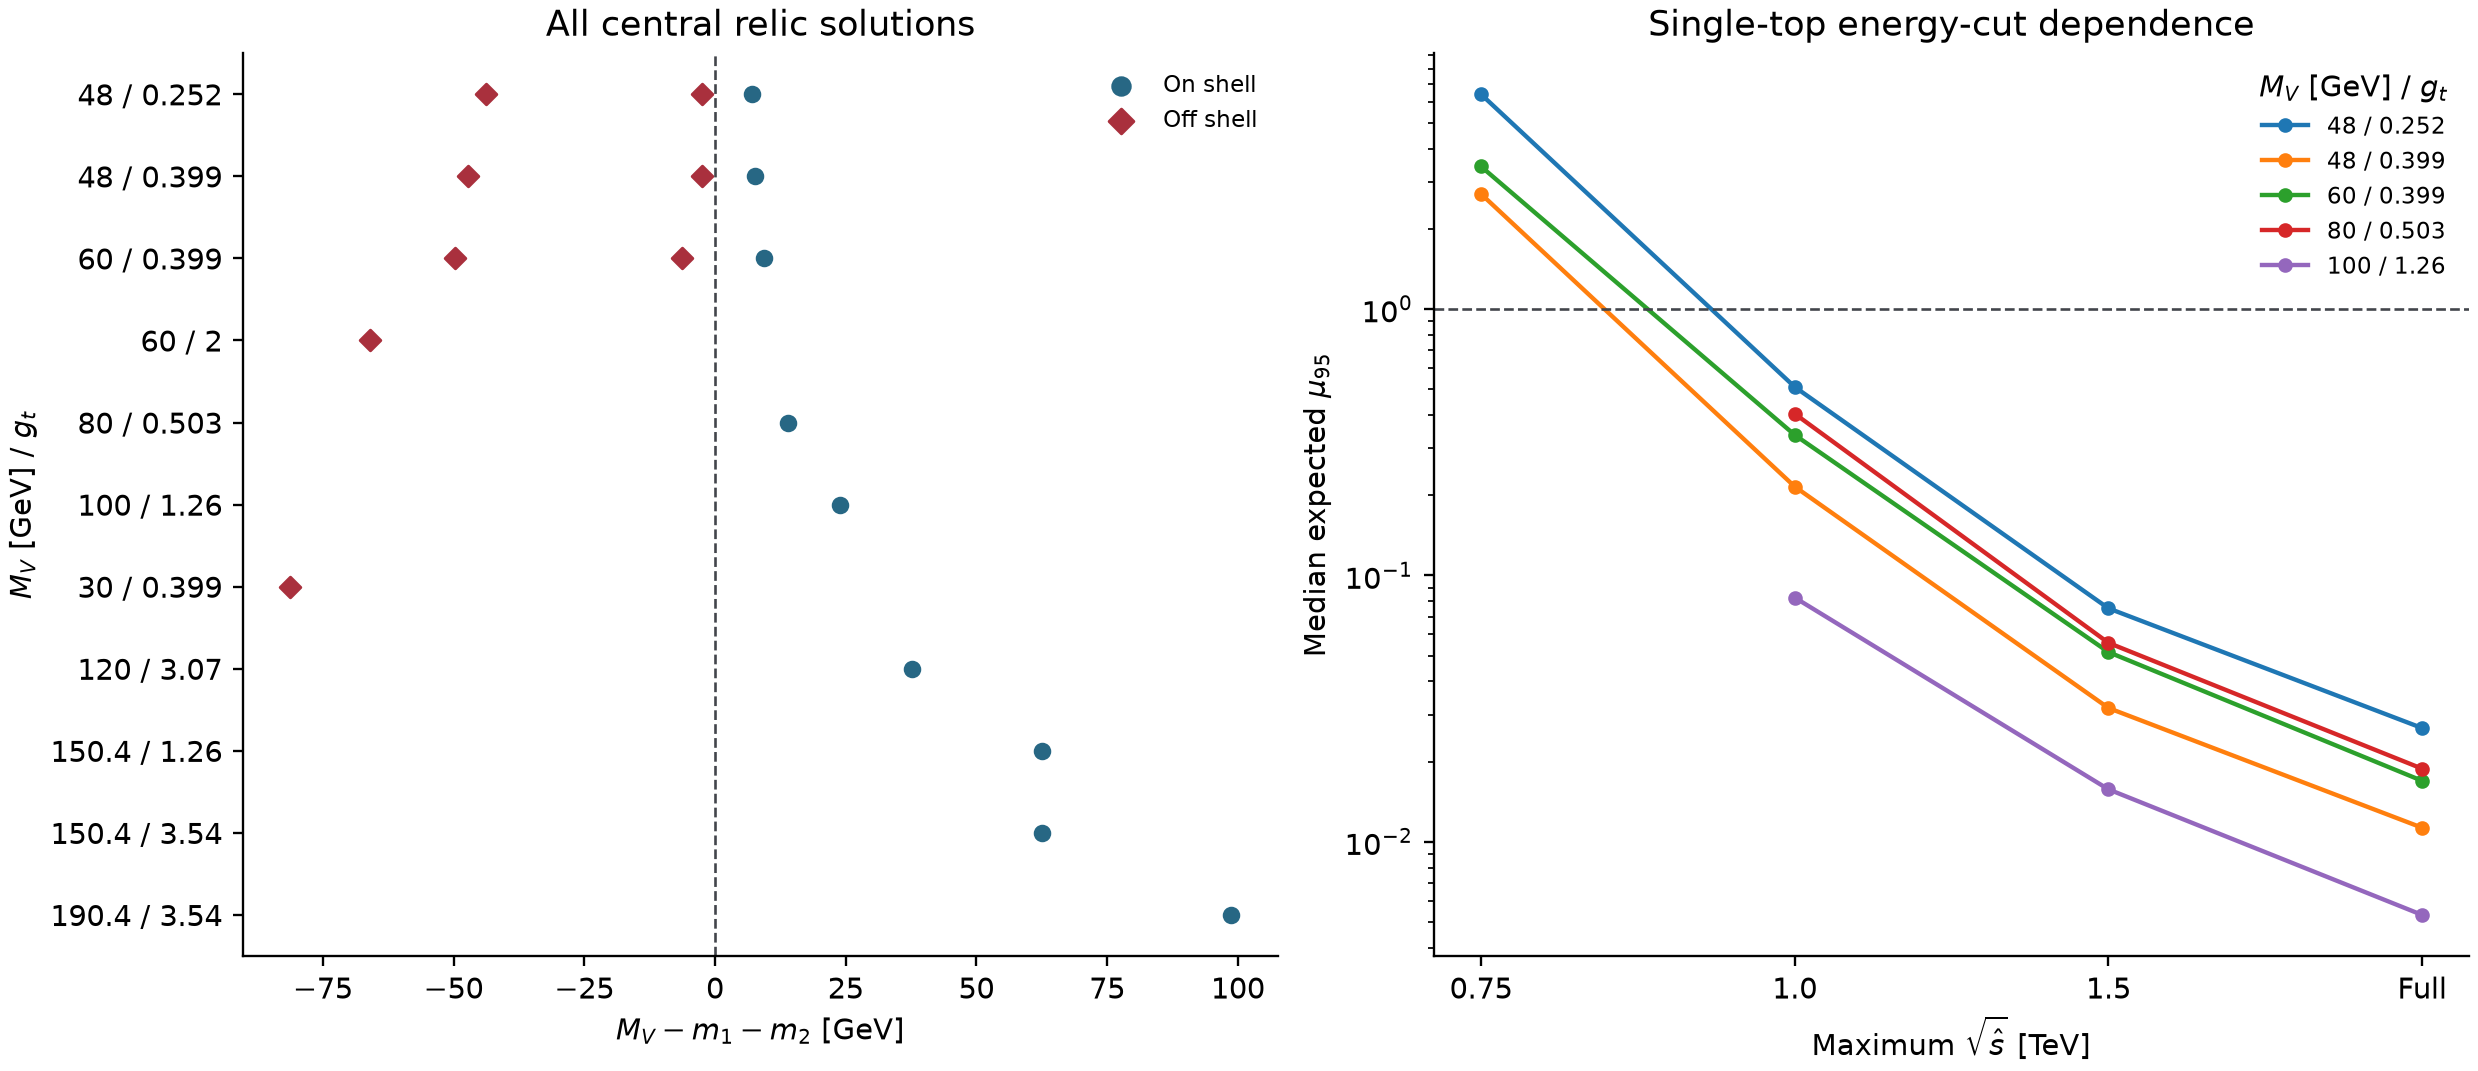
\includegraphics[width=.86\linewidth]{figures/08_top_branches_and_energy.png}
\caption{The left panel shows $M_V-m_1-m_2$ at representative central relic solutions. The right panel shows how the expected single-top sensitivity varies with the partonic-energy cut for on-shell solutions. The charged weak current connects top and bottom quarks with different $V$ couplings, so the high-energy behavior of longitudinal weak-boson amplitudes depends on cancellations in the electroweak completion. Varying the cut probes that dependence. Missing markers at 0.75 TeV indicate samples for which the approximate likelihood gives no finite limit.}
\label{fig:single_top_cut}
\end{figure}

\subsection{Low-mass branches and truth-level rates}

\begin{figure}[tbp]
\centering
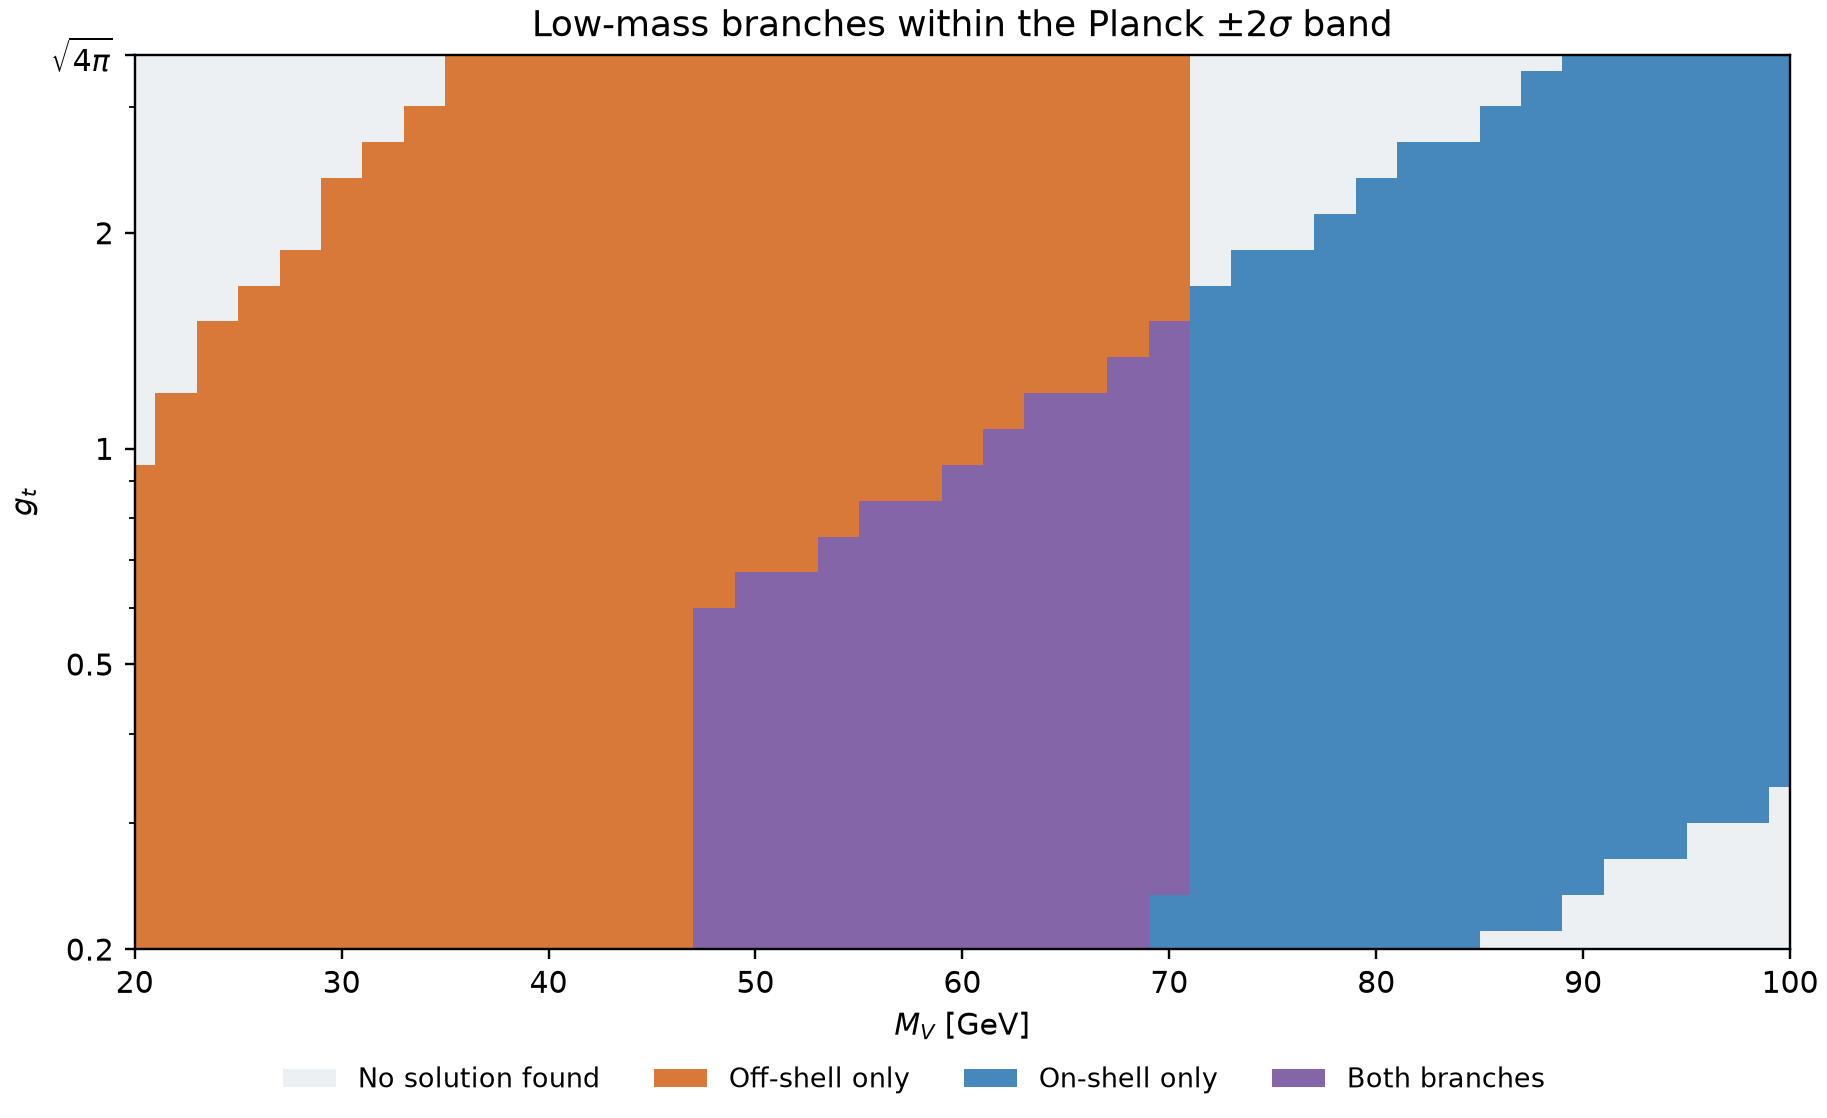
\includegraphics[width=.58\linewidth]{figures/d01_light_top_branches.png}
\caption{Independent low-mass scan with tree-level yield matching. Colors identify the relic branches found within the Planck $\pm2\sigma$ band. Purple indicates that both on-shell and off-shell solutions are present.}
\label{fig:low_mass}
\end{figure}

\begin{figure}[tbp]
\centering
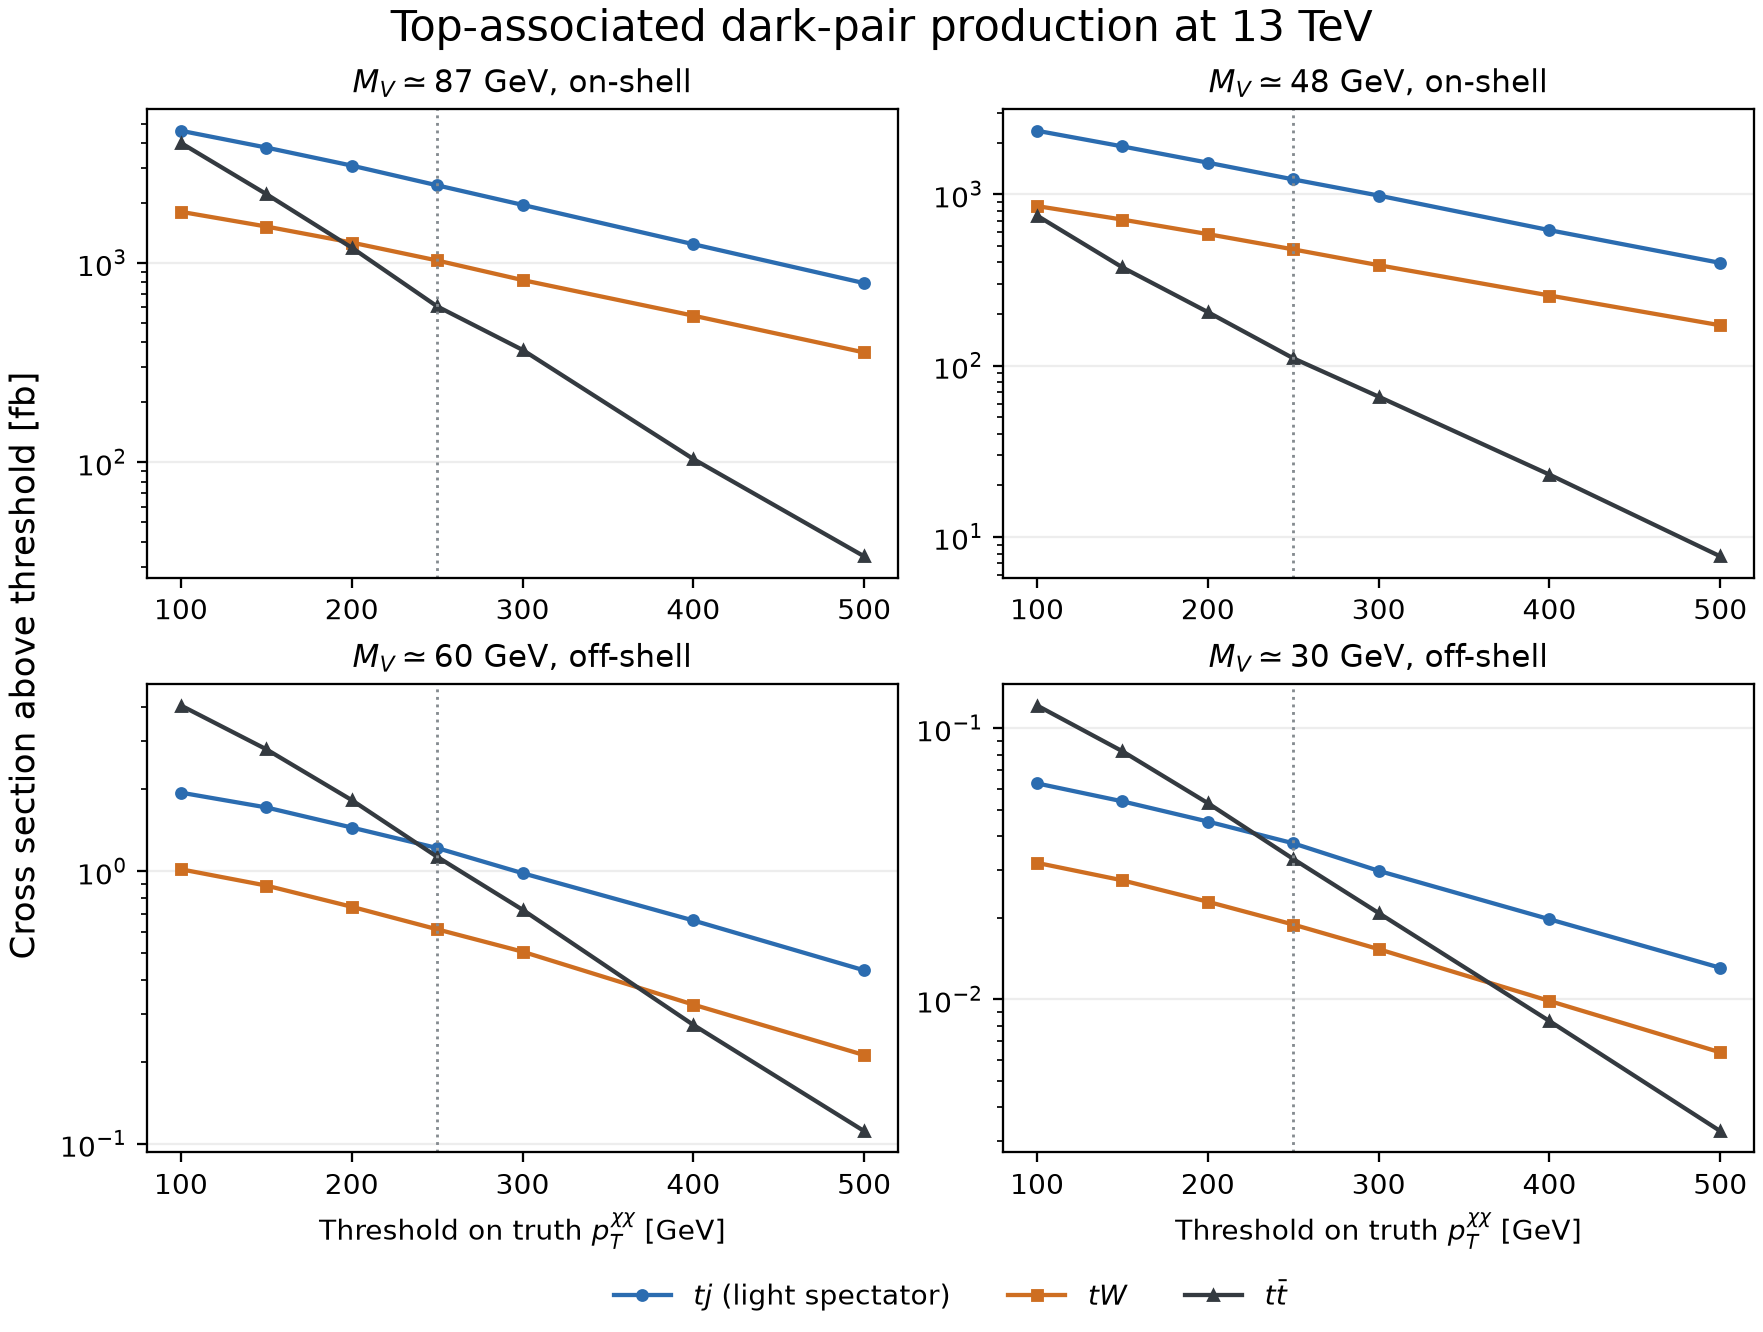
\includegraphics[width=.86\linewidth]{figures/d02_top_truth_met.png}
\caption{Cross sections in fb above different truth-level MET thresholds for dark-pair production with $tj$, $tW$, or $t\bar t$ at four on-shell or off-shell benchmarks. Deriving experimental limits requires simulating top decays and validating reconstruction and selection efficiencies at the same parameter points.}
\label{fig:top_truth_met}
\end{figure}

For $m_\chi\ge20$ GeV and $M_V\le40.001$ GeV, dark-pair production proceeds through an off-shell mediator. To derive a top-pair exclusion from fully simulated samples, one must check $m_\chi$, the decay threshold, and the template normalization at each point with a common reference yield. The published CMS backgrounds come from a simultaneous fit that includes signal-region data. An observed recast requires background constraints independent of the signal-region counts. \cite{cmstop}


\clearpage
\twocolumngrid
\bibliography{references}
\end{document}
